% =========================
% COMP 499/691 Progress Report (CVPR-style template)
% =========================

\documentclass[10pt,twocolumn,letterpaper]{article}

\usepackage[review]{cvpr}
\usepackage{graphicx}
\usepackage{amsmath,amssymb}
\usepackage{booktabs}
\usepackage[pagebackref,breaklinks,colorlinks]{hyperref}
\usepackage[capitalize]{cleveref}
\crefname{section}{Sec.}{Secs.}
\Crefname{section}{Section}{Sections}
\Crefname{table}{Table}{Tables}
\crefname{table}{Tab.}{Tabs.}

\title{COMP 499 Progress Report:\\Lung Histopathology Classification on LungHist700}

\begin{document}
\maketitle

% =========================
\section{Introduction and Problem Statement}
\label{sec:intro}

Lung cancer histopathology classification is a clinically relevant computer vision problem: automated tissue image interpretation can support pathologists by accelerating routine screening and improving diagnostic consistency. The primary challenges in the literature include (i)~\textbf{limited labeled data} — public lung histopathology datasets typically contain only a few hundred images, making model generalization difficult; (ii)~\textbf{patient-level leakage} — patches from the same patient are highly correlated, inflating performance if splits are done at the patch rather than patient level; (iii)~\textbf{weak supervision} — clinical labels annotate entire slides, not individual patches, motivating multiple-instance learning (MIL); and (iv)~\textbf{domain gap} — ImageNet-pretrained features do not fully capture H\&E stain morphology. Common mitigations include patient-wise splitting, class weighting, transfer learning from pretrained convolutional networks, and aggregation-based MIL.

Our project evaluates four approaches on LungHist700~\cite{lunghist700paper} (691 high-resolution histopathology images, 20$\times$/40$\times$ magnification) in a three-class setting: adenocarcinoma (ACA), normal (NOR), and squamous cell carcinoma (SCC). We aim to (i)~reproduce the ResNet50 patch-level CNN baseline and compare with published benchmarks, (ii)~implement an end-to-end MIL pipeline, (iii)~implement frozen-backbone MIL with multi-head self-attention and gated attention aggregators, and (iv)~report accuracy, macro-F1, and ROC-AUC with confusion matrices and learning curves. We expect the patch-level CNN to outperform MIL in raw accuracy due to its denser supervision, and frozen-backbone MIL with gated attention to approach end-to-end MIL performance at much lower training cost.

% =========================
\section{Proposed Methodologies}
\label{sec:method}

\textbf{Dataset and Splits.}
LungHist700 comprises 691 images (1200$\times$1600~px) across seven sub-classes grouped into three superclasses (ACA, NOR, SCC). Patient-wise splitting ensures no patient ID overlaps across train/val/test. Class-weighted cross-entropy reduces majority-class bias.

\textbf{CNN Baseline (ResNet50).}
A ResNet50 backbone pretrained on ImageNet is fine-tuned for 3-way classification. Images are resized to 300$\times$400 and randomly cropped to 224$\times$224 at training time. We monitor accuracy, macro-F1, AUC, and per-class confusion matrices; Grad-CAM visualizations assess qualitative saliency (see \textbf{Supplement~A}).

\textbf{End-to-End MIL (ResNet50 + Multi-Head Self-Attention).}
Each slide is treated as a \emph{bag} of 20 randomly sampled 224$\times$224 patches from the full-resolution image, following the original paper's bag construction~\cite{lunghist700paper}. A shared ResNet50 backbone encodes each patch into a 2048-dim embedding; a 4-head self-attention module aggregates patch embeddings before a linear classifier. The entire network trains jointly under bag-level labels. Attention weight maps identify the most discriminative patches (see \textbf{Supplement~C}).

\textbf{Frozen-Backbone MIL (Offline Embeddings).}
To address training instability, we freeze the ResNet50 and pre-compute 2048-dim embeddings for a deterministic 5$\times$7 grid of 35 patches per image, enabling offline caching. Two lightweight aggregators are then trained:
(a)~\textbf{Multi-Head Self-Attention} — 4-head self-attention with mean-pooling;
(b)~\textbf{Gated Attention}~\cite{ilse2018} — per-patch sigmoid-tanh gating with weighted-sum aggregation.
Training curves for both are in \textbf{Supplement~B}.

% =========================
\section{Attempts at Solving the Problem}
\label{sec:attempts}

\textbf{Environment and Reproducibility.}
Local setup required resolving CUDA/cuDNN library visibility under WSL, TensorFlow–protobuf version alignment, and missing dataset path defaults. A critical MIL bug — patches extracted from a downscaled 300$\times$400 image rather than the full 1200$\times$1600 original — was identified and corrected, restoring micro-texture information critical for the attention mechanism.

\textbf{CNN Baseline Results.}
The CNN achieves \textbf{Acc 91.7\%, AUROC 99.5\%, Macro-F1 0.915}, matching the paper's $\approx$90\%/98\% benchmark (Tab.~\ref{tab:all_results}). NOR is classified near-perfectly; ACA/SCC confusion is the main error mode, consistent with overlapping glandular/squamous morphology. See \textbf{Supplement~A} for training curves and confusion matrix.

\textbf{End-to-End MIL Results.}
The jointly trained backbone+attention model reaches \textbf{Acc 70.8\%, AUROC 91.3\%, Macro-F1 0.701}. Accuracy is $\approx$10 points below the paper's MIL figure (81\%) due to cold-start instability (attention and backbone optimised simultaneously), gradient noise from 25M parameters under a single bag label, and a small training set ($\approx$560 bags). Notably, \textbf{AUROC 91.3\% exceeds the paper's 89\%}, indicating well-calibrated class probabilities. Attention visualizations confirm the model focuses on morphologically relevant patch regions (Supplement~C).

\textbf{Frozen-Backbone MIL Results.}
Results are in \cref{tab:all_results}. \textbf{Gated attention} (Acc 70.8\%, AUROC 86.6\%) matches end-to-end MIL accuracy while training orders of magnitude faster. Its sparse per-patch gating is better regularised than self-attention given only $\sim$560 training bags. \textbf{Multi-head self-attention} (Acc 68.75\%, AUROC 86.1\%) underperforms — its higher parameter count leads to overfitting in the small-data regime, and SCC recall collapses to 36\%. SCC is the critical failure class across all MIL variants (36–55\% recall), pointing to the ImageNet domain gap as the primary bottleneck.

\begin{table}[h]
\centering
\caption{All models vs.\@ published paper benchmarks (20$\times$, 3-class).}
\label{tab:all_results}
\setlength{\tabcolsep}{4pt}
\begin{tabular}{lccc}
\toprule
Model & Acc & AUROC & F1 \\
\midrule
Paper CNN~\cite{lunghist700paper}       & 0.90 & 0.98 & --- \\
\textbf{Ours — CNN ResNet50}            & \textbf{0.917} & \textbf{0.995} & \textbf{0.915} \\
\midrule
Paper MIL~\cite{lunghist700paper}       & 0.81 & 0.89 & --- \\
Ours — End-to-End MIL                   & 0.708 & 0.913 & 0.701 \\
Ours — Frozen (Gated Attn)              & 0.708 & 0.866 & 0.700 \\
Ours — Frozen (Self-Attn)              & 0.688 & 0.861 & 0.647 \\
\bottomrule
\end{tabular}
\end{table}

\textbf{Key finding:} CNN $>$ all MIL variants in accuracy, confirming the paper's conclusion. The accuracy advantage of patch-level supervision diminishes when slide-level labels are the only available annotation, motivating frozen-backbone MIL as a practical alternative.

% =========================
\section{Future Steps}
\label{sec:future}

\begin{enumerate}
\item \textbf{Domain-adapted backbone:} Replace ImageNet ResNet50 with a histopathology-specific encoder (UNI, CONCH, or PLIP) to close the feature domain gap and improve SCC recall.
\item \textbf{Vision Transformer (ViT):} Evaluate ViT (default and fine-tuned) as backbone for both patch-level and frozen-MIL pipelines.
\item \textbf{Interpretability:} Extend Grad-CAM (CNN) and attention heatmaps (MIL) to verify alignment with pathologist-defined discriminative regions.
\item \textbf{Statistical validation:} Report mean $\pm$ std over multiple random seeds to quantify variance in the small-data regime.
\item \textbf{40$\times$ experiments:} Replicate the full pipeline at 40$\times$ magnification to assess resolution sensitivity.
\end{enumerate}

% =========================
\section*{References}
\begin{thebibliography}{9}

\bibitem{lunghist700paper}
J. Marino, S. Khan \etal\
LungHist700: A Dataset of Histological Images for Deep Learning in Pulmonary Pathology.
\textit{Scientific Data}, 2024.

\bibitem{lunghist700}
LungHist700 open-source repository.
\url{https://github.com/jorgediosdado/LungHist700}

\bibitem{skattoju}
S. Kattoju. LungHist700 PyTorch reimplementation and MIL extensions.
\url{https://github.com/skattoju/LungHist700/}

\bibitem{resnet}
K. He, X. Zhang, S. Ren, J. Sun.
Deep Residual Learning for Image Recognition.
\textit{CVPR}, 2016.

\bibitem{ilse2018}
M. Ilse, J. Tomczak, M. Welling.
Attention-based Deep Multiple Instance Learning.
\textit{ICML}, 2018.

\bibitem{chen2022}
R. J. Chen \etal\
Scaling Vision Transformers to Gigapixel Images via Hierarchical Self-Supervised Learning.
\textit{CVPR}, 2022.

\end{thebibliography}

% =======================================================================
% SUPPLEMENTARY MATERIAL — not subject to page limit
% =======================================================================
\newpage
\onecolumn
\section*{Supplementary Material}

\noindent This appendix supports the main report with full training curves, confusion matrices, qualitative visualizations, and environment details.

% -----------------------------------------------------------------------
\subsection*{A\quad CNN ResNet50 Baseline — Training Curves and Evaluation}
% -----------------------------------------------------------------------

\begin{figure}[h]
\centering
\begin{tabular}{ccc}
  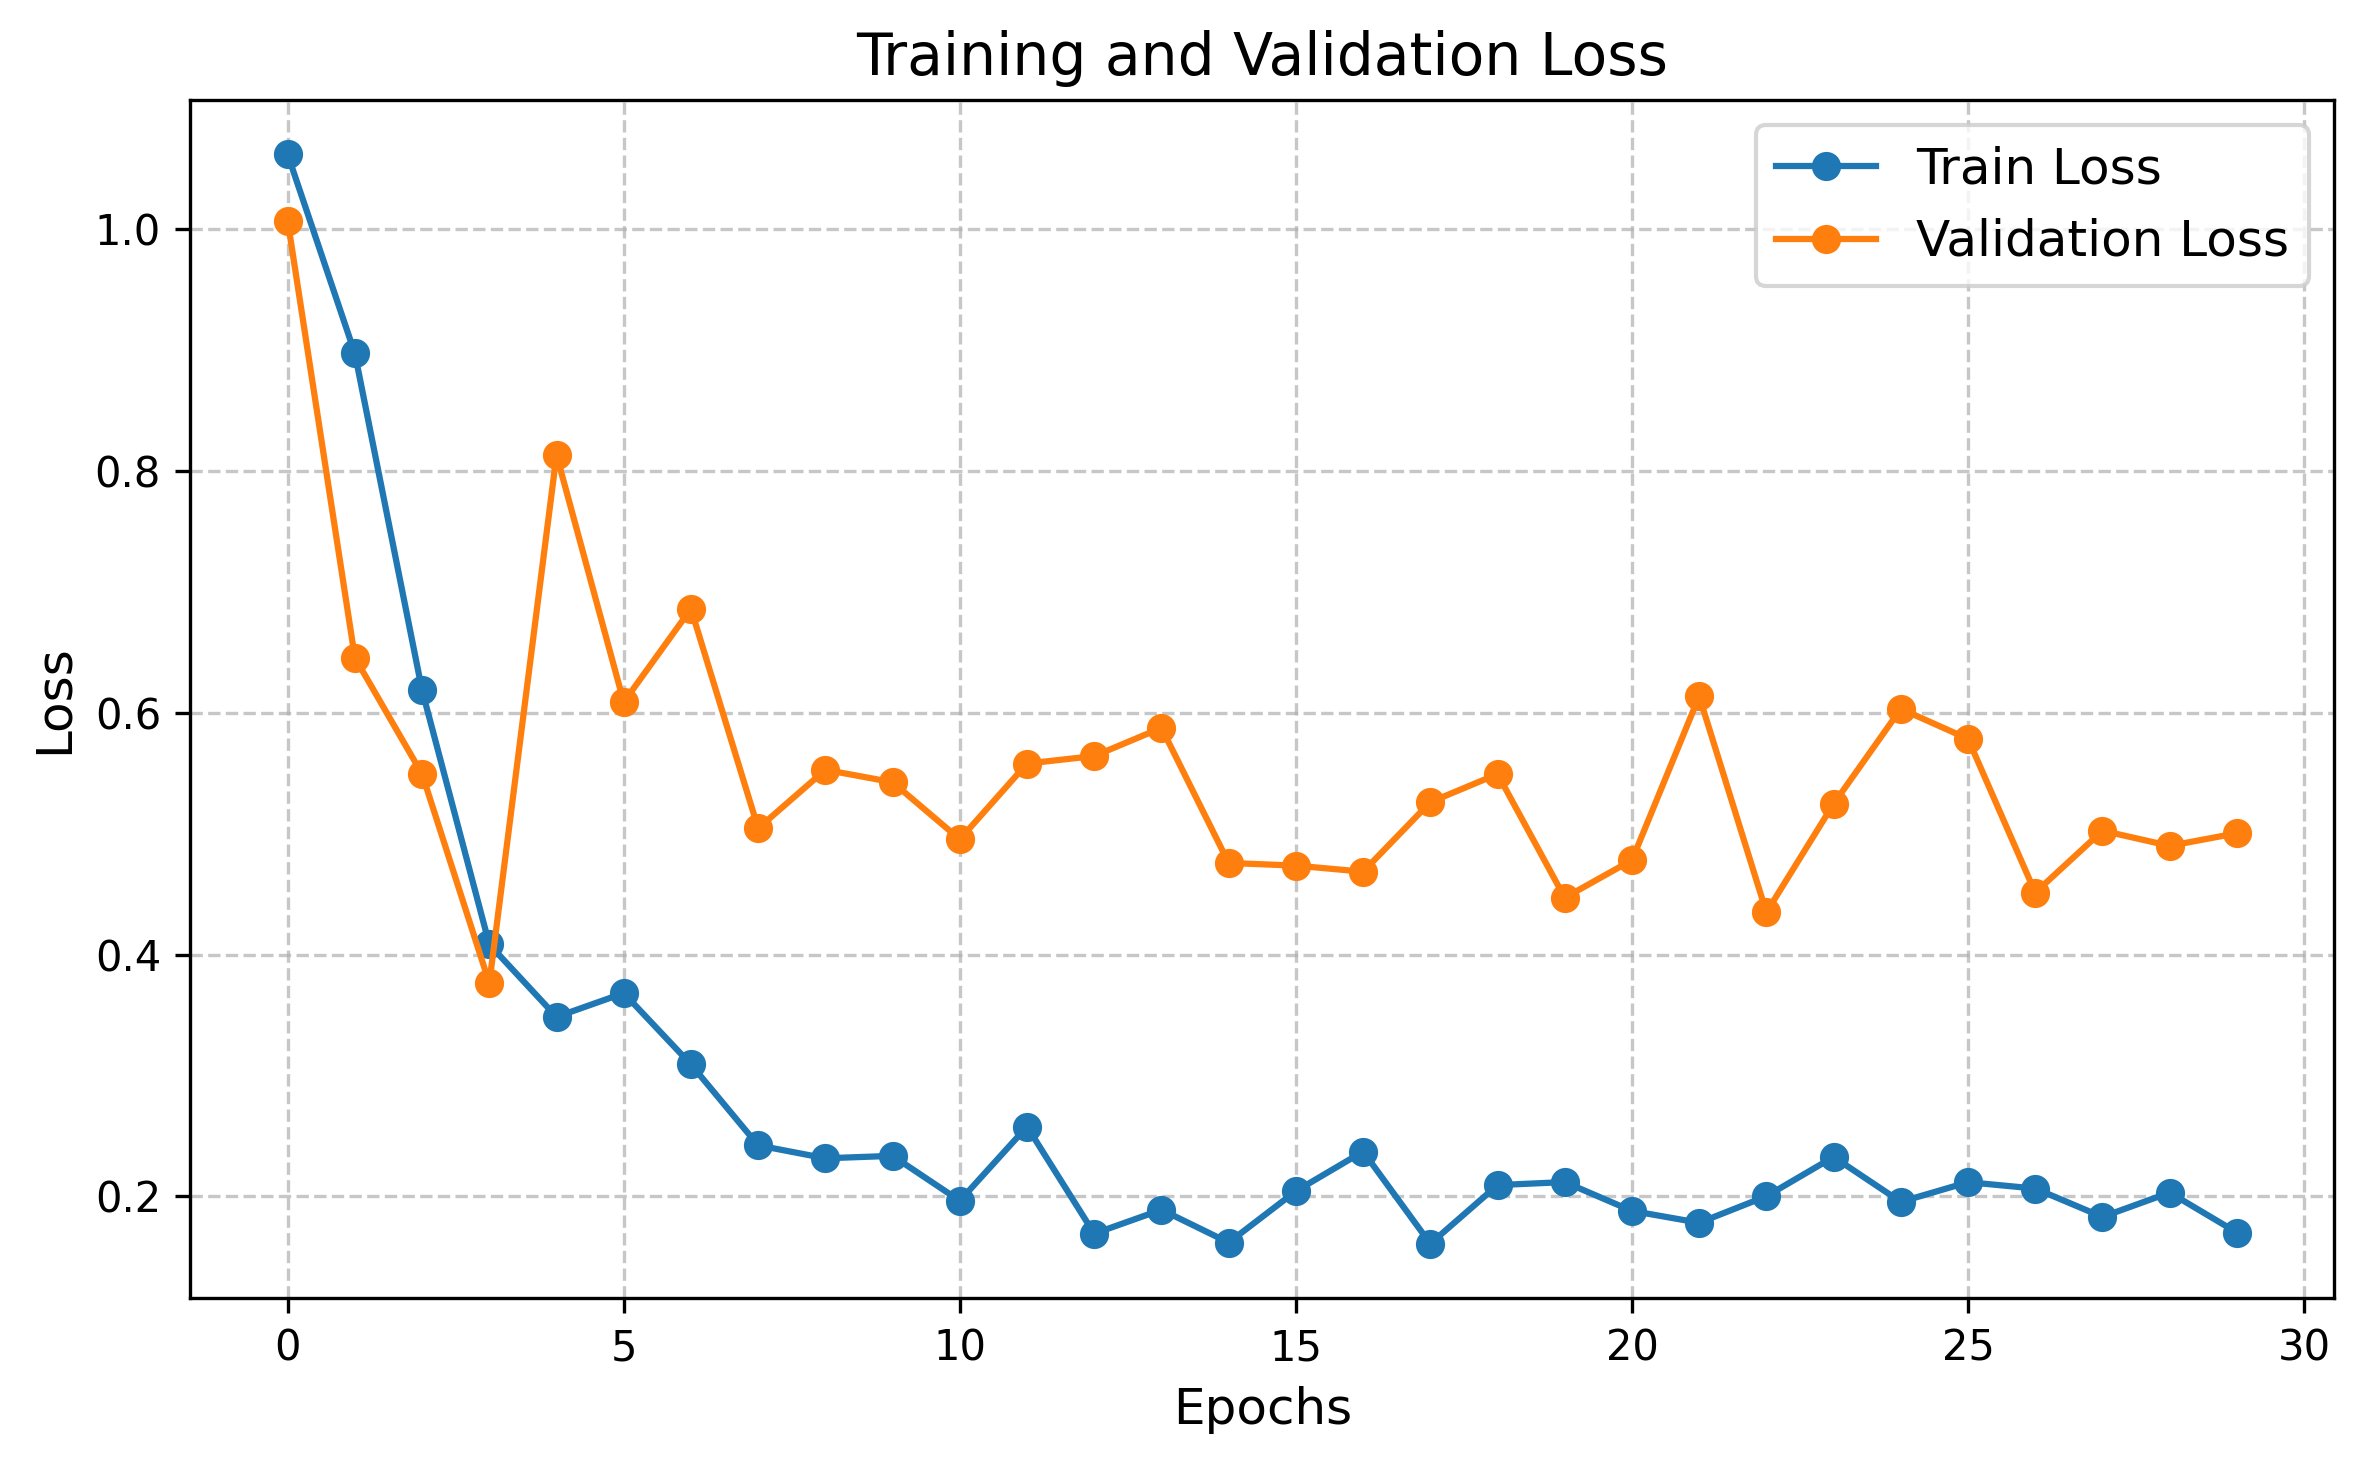
\includegraphics[width=0.31\textwidth]{baseline_loss.png} &
  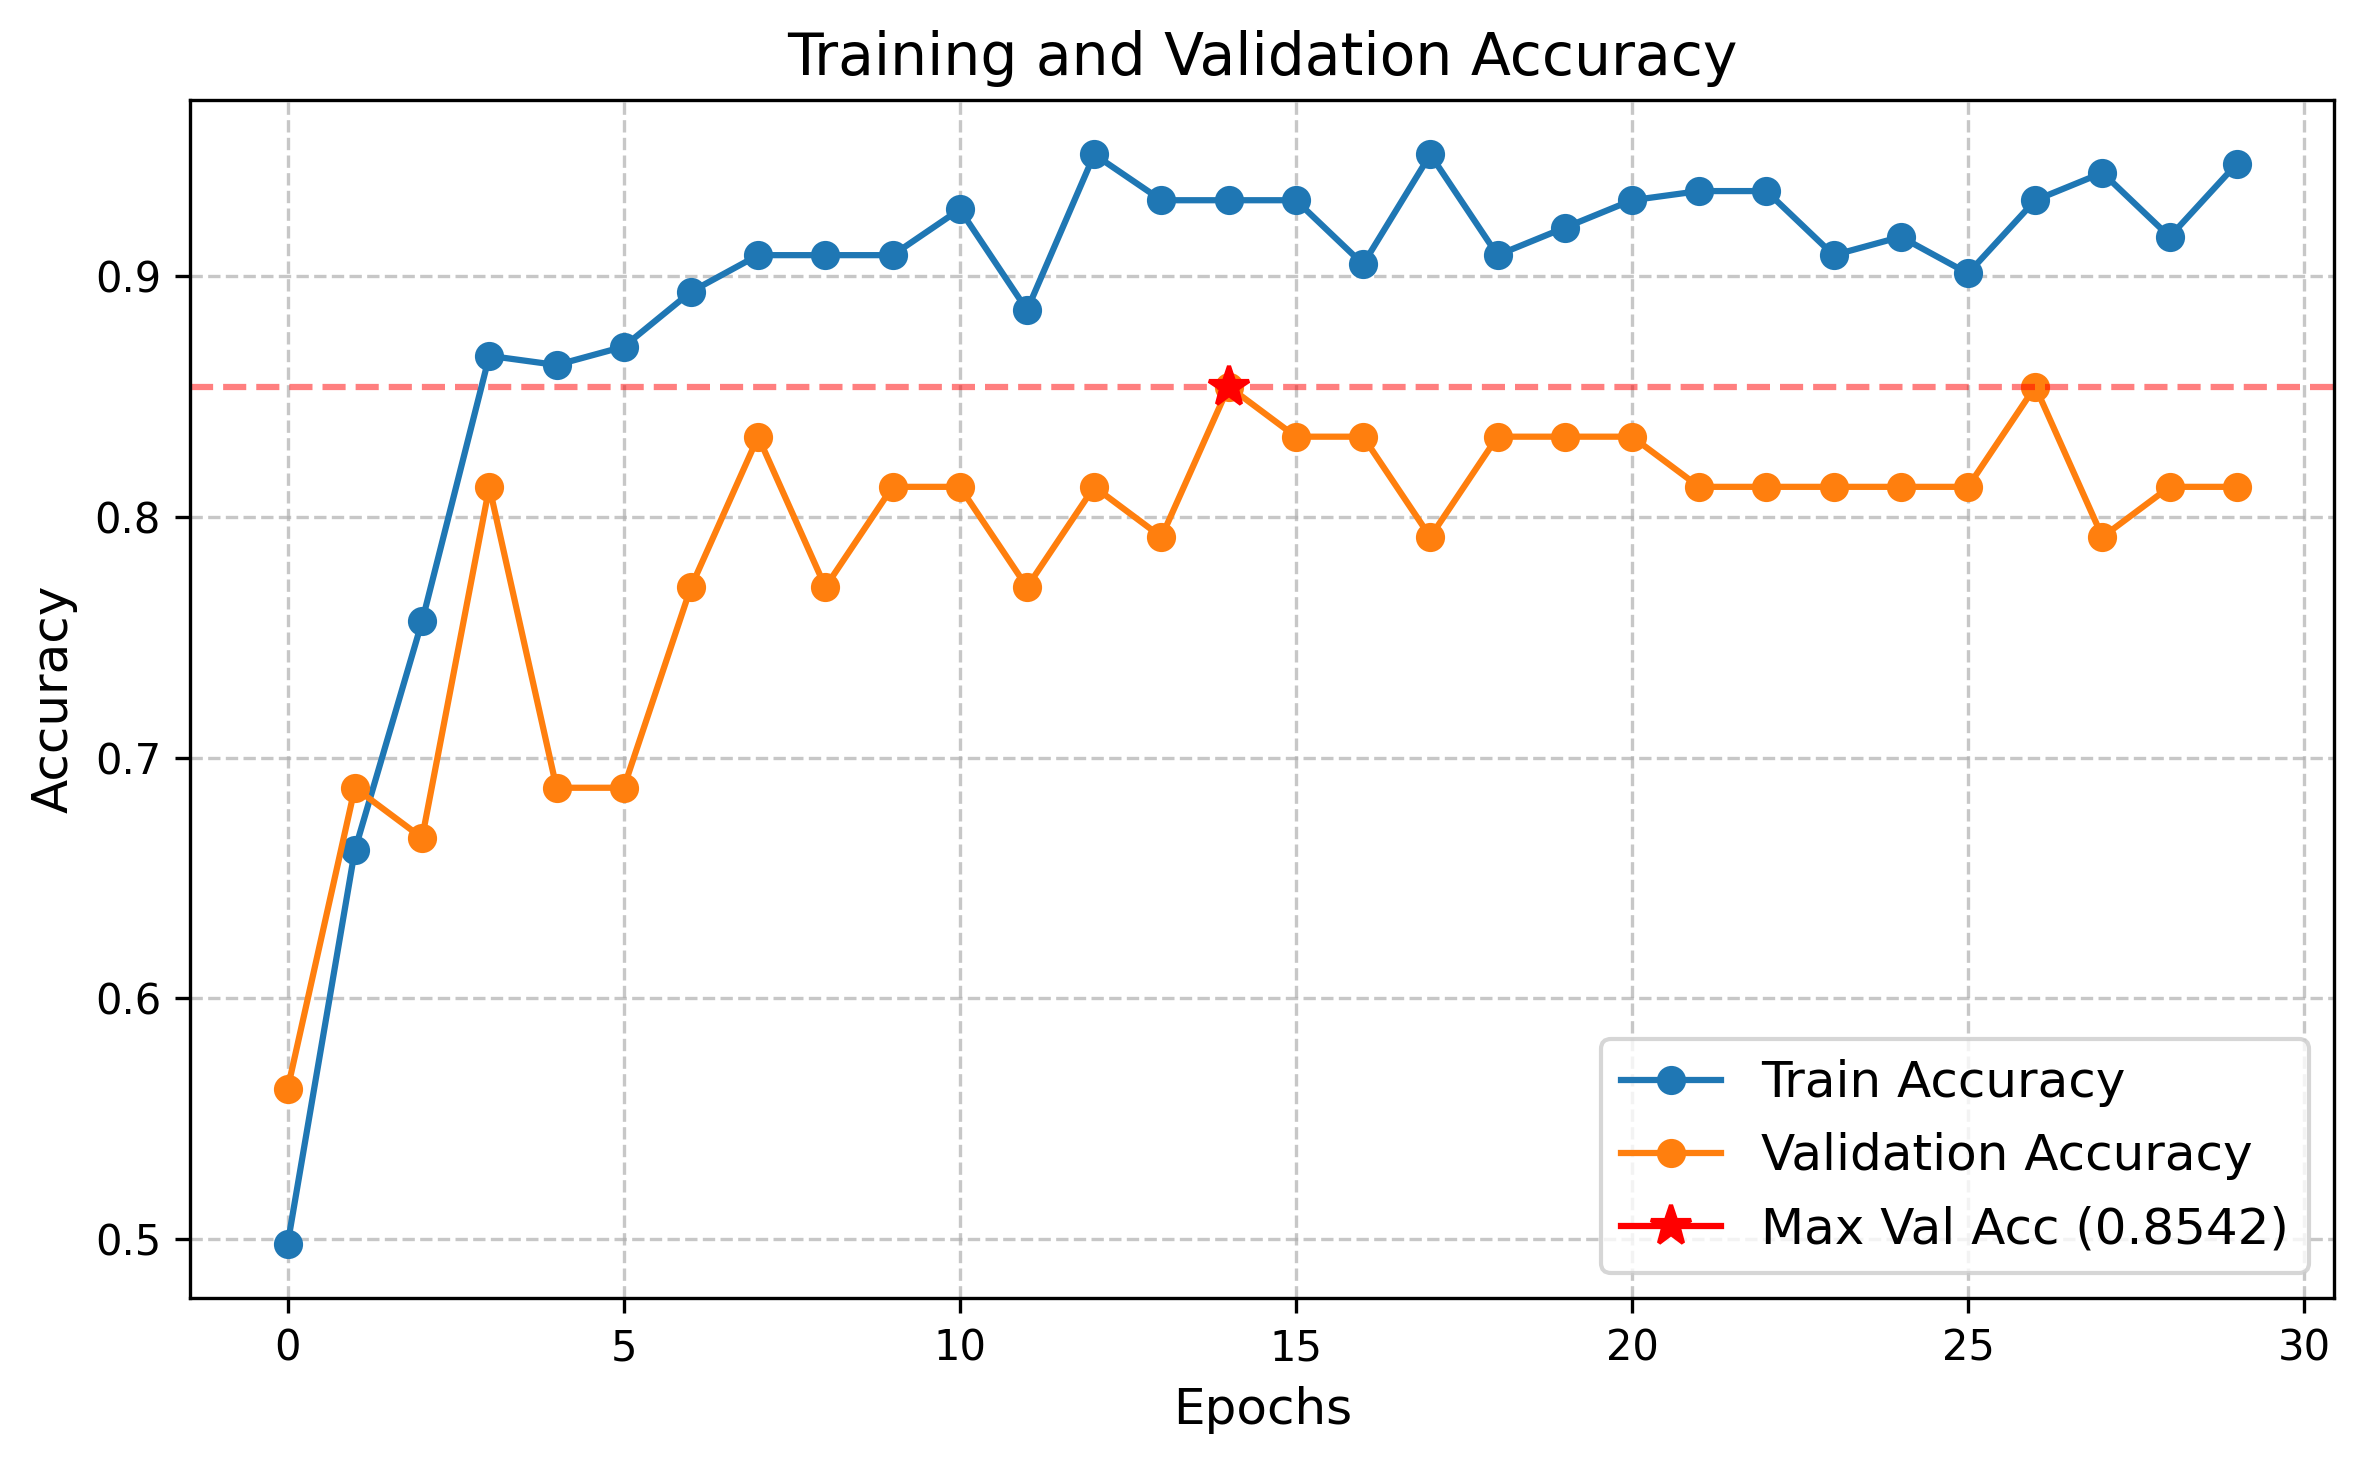
\includegraphics[width=0.31\textwidth]{baseline_accuracy.png} &
  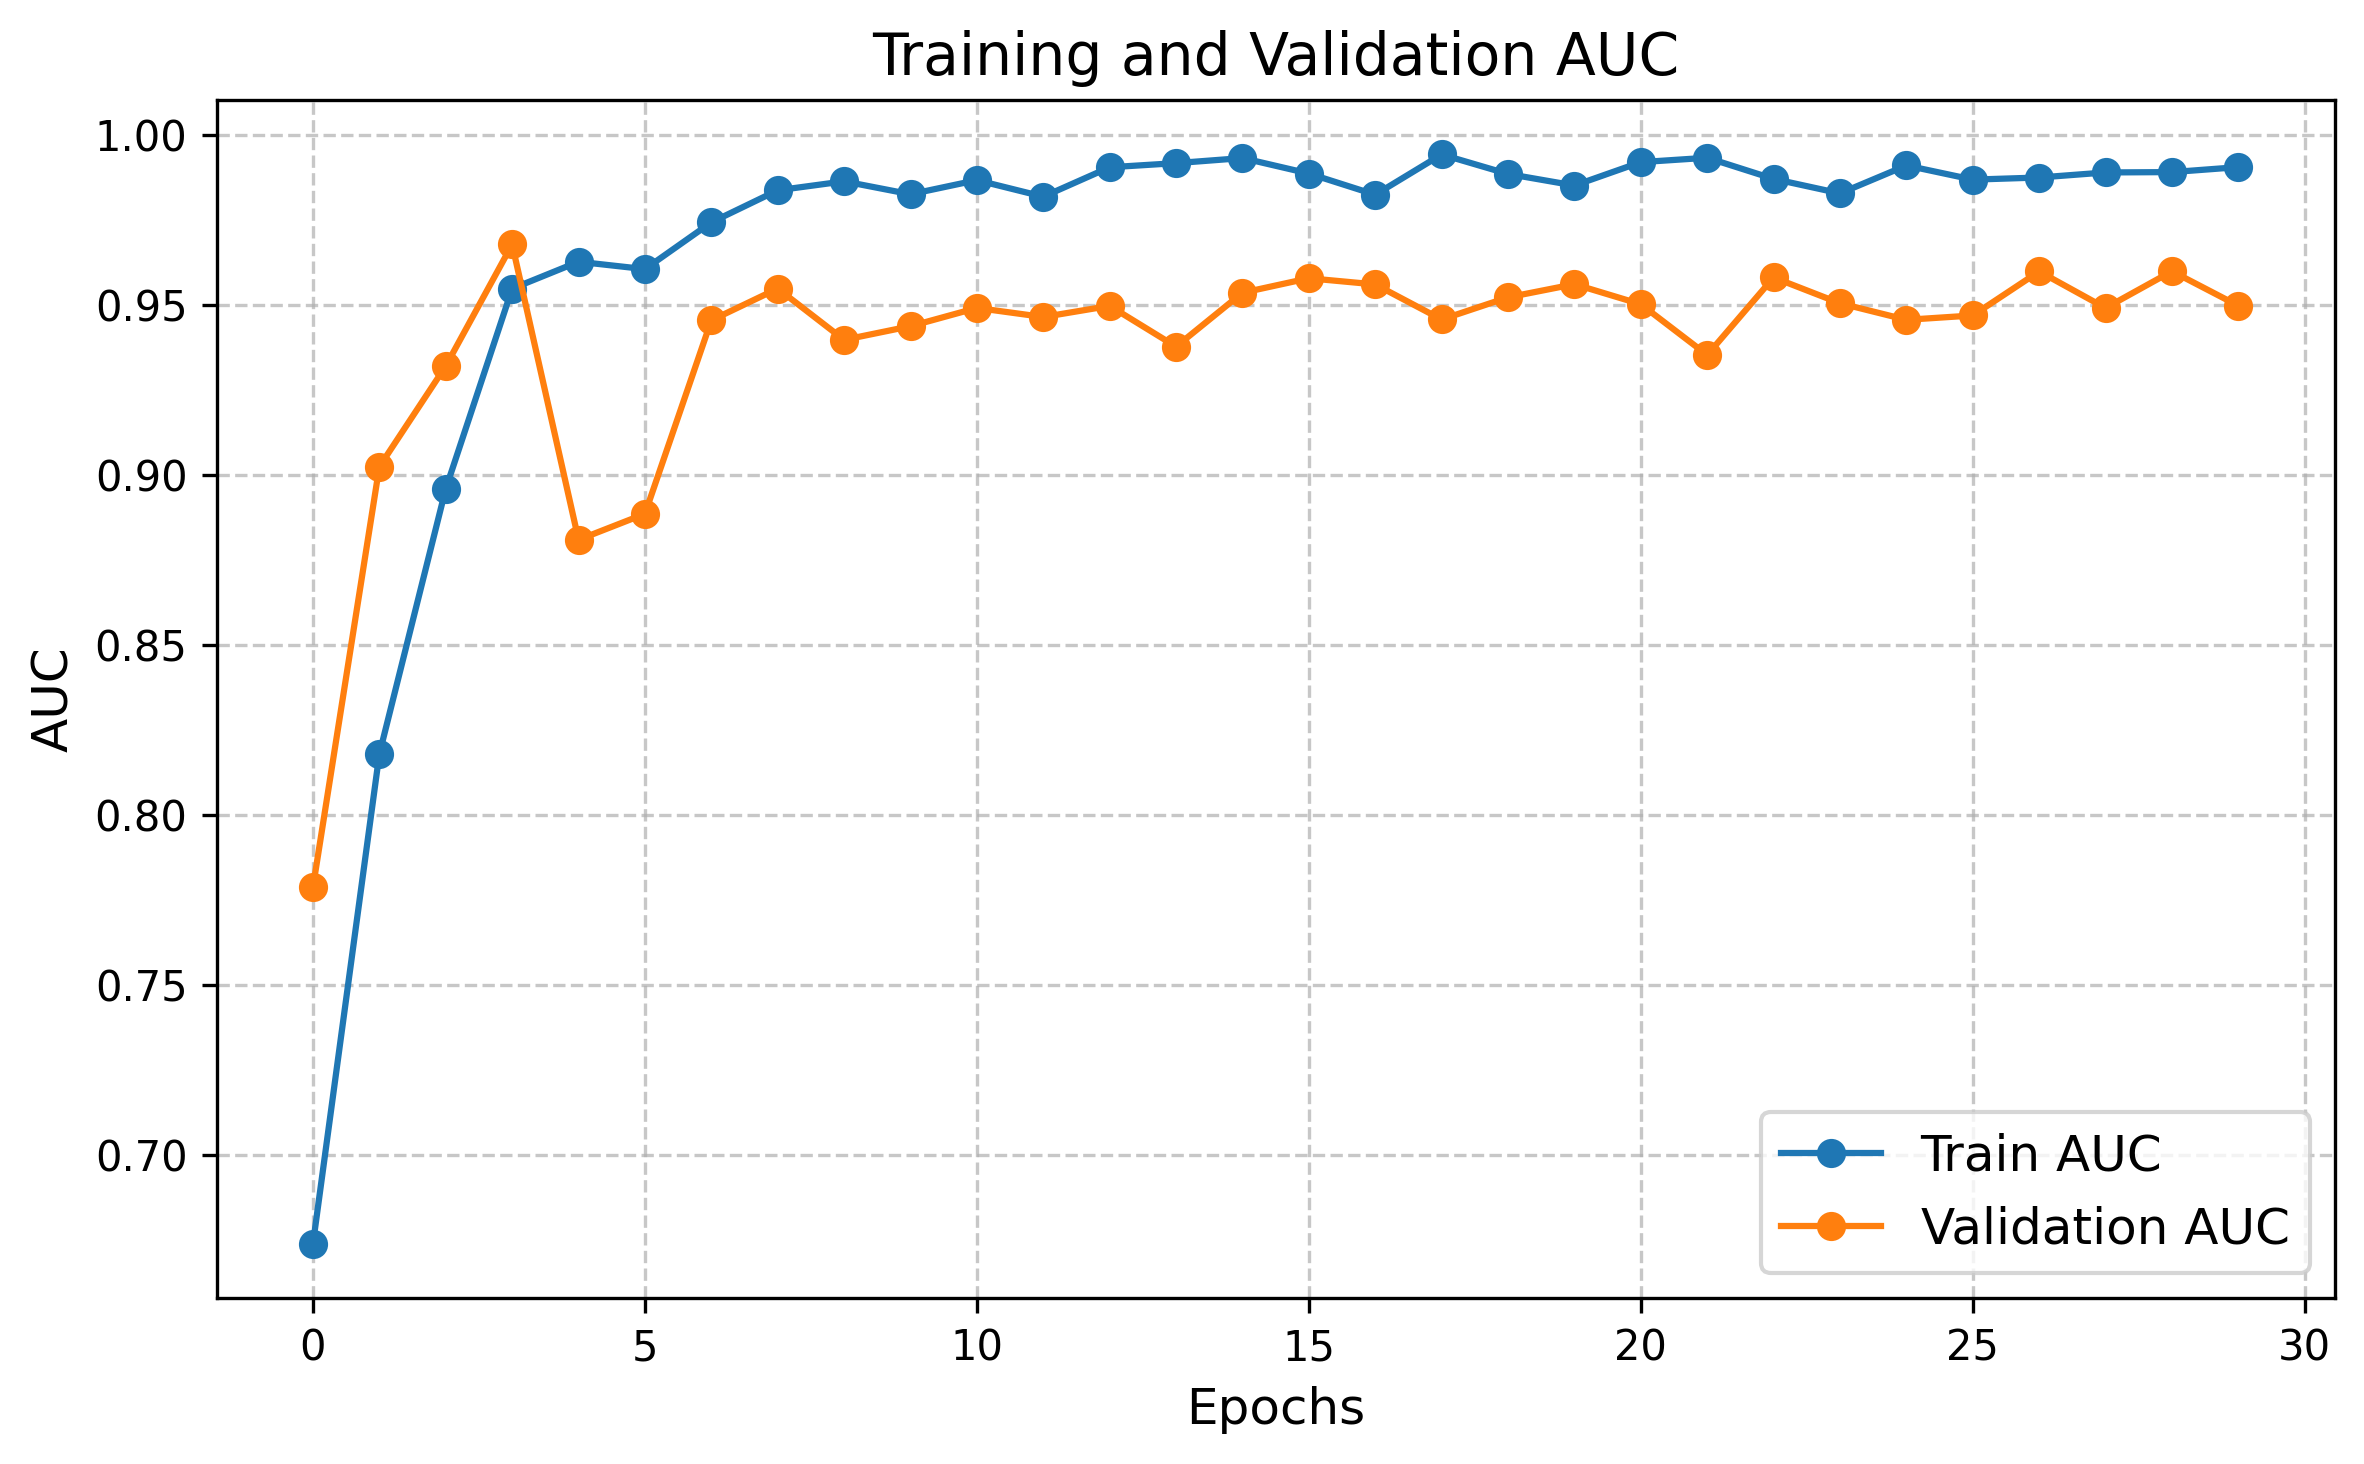
\includegraphics[width=0.31\textwidth]{baseline_auc.png}
\end{tabular}
\caption{\textbf{CNN Baseline training curves.} Left: Loss — rapid convergence, minimal train/val gap. Centre: Accuracy — star marks best val accuracy epoch. Right: AUROC — consistently high throughout training.}
\label{fig:cnn_curves}
\end{figure}

\begin{figure}[h]
\centering
\begin{tabular}{cc}
  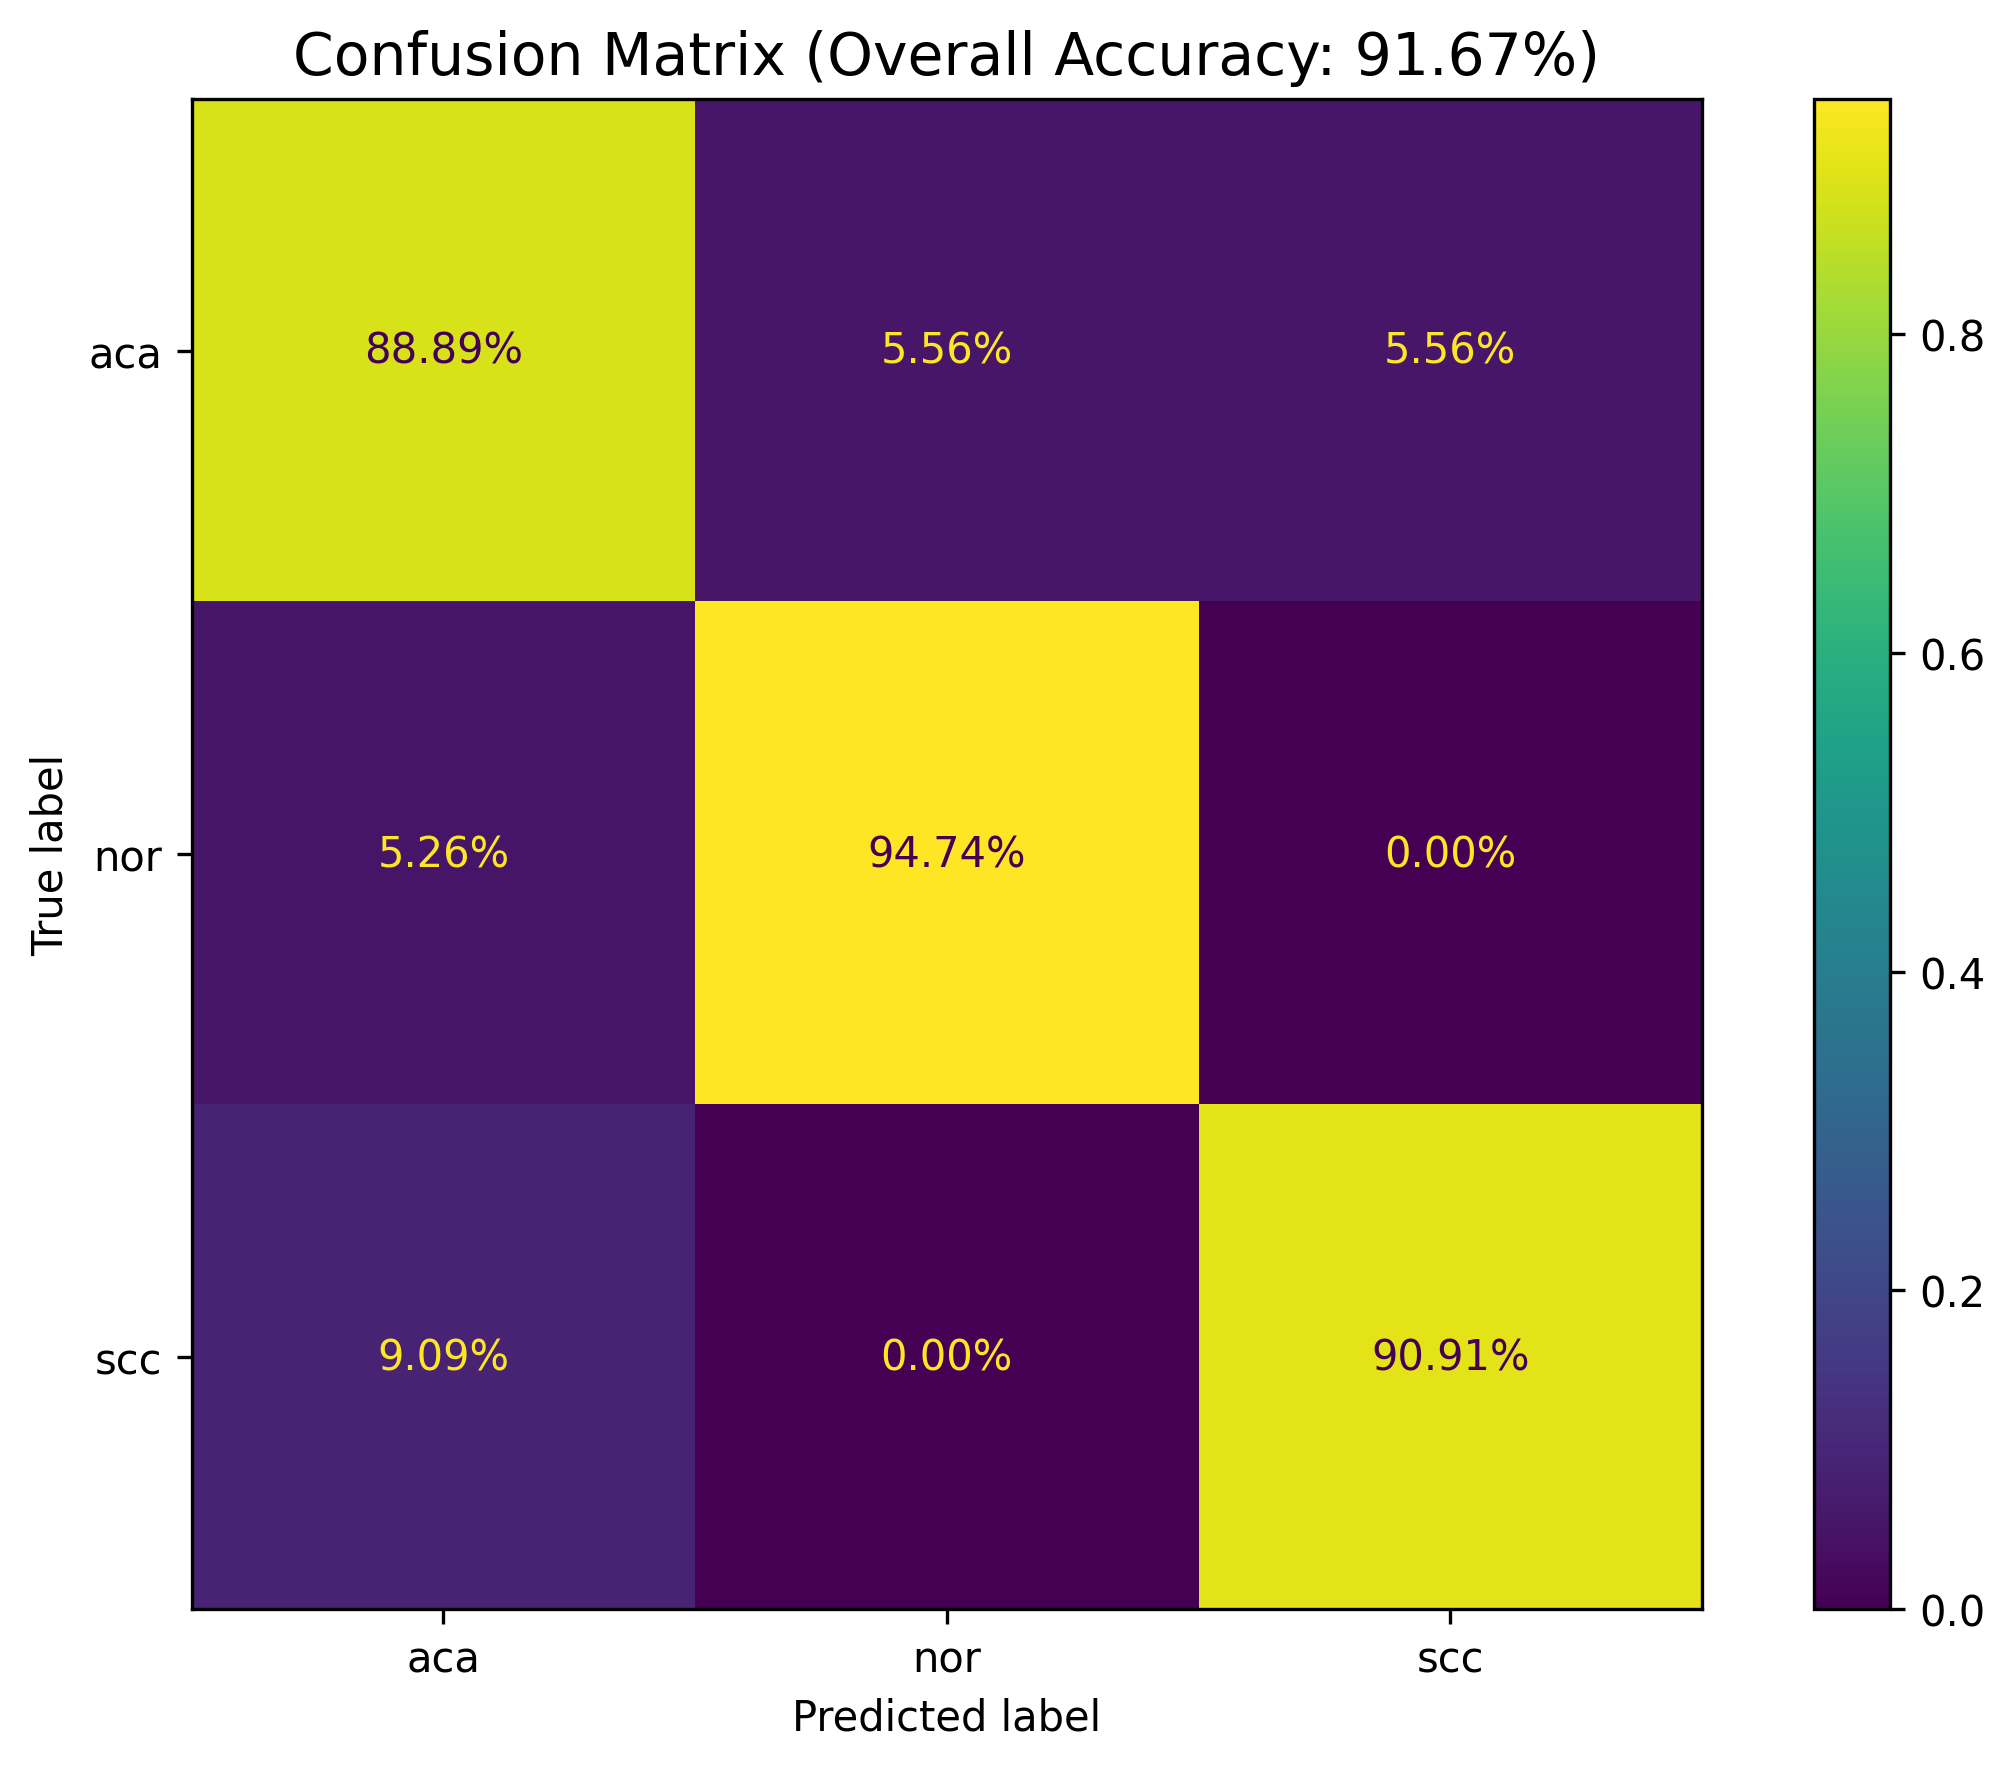
\includegraphics[width=0.42\textwidth]{baseline_confusion_matrix.png} &
  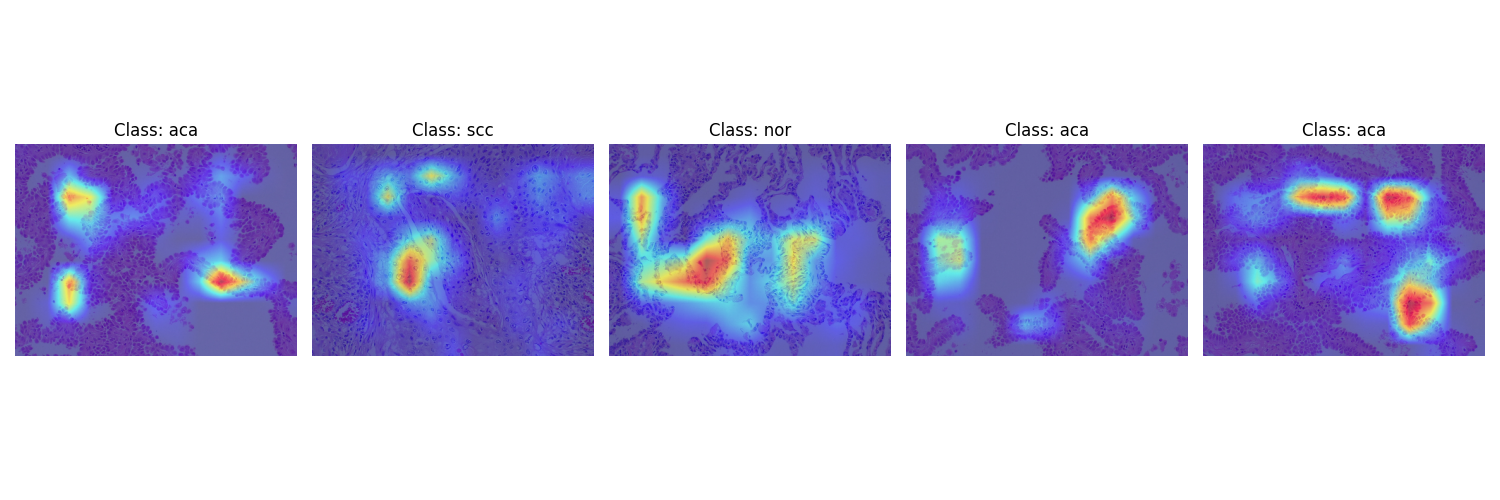
\includegraphics[width=0.52\textwidth]{gradcam_samples.png}
\end{tabular}
\caption{\textbf{CNN evaluation.} Left: Normalized confusion matrix (per-class recall). NOR is classified near-perfectly; the main confusion is between ACA and SCC, reflecting overlapping glandular morphology. Right: Grad-CAM activation maps on validation samples — the model attends to tissue architecture (glandular lumina, nuclear patterns) rather than background stroma.}
\label{fig:cnn_eval}
\end{figure}

% -----------------------------------------------------------------------
\subsection*{B\quad Frozen ResNet50 MIL — Training Curves and Confusion Matrices}
% -----------------------------------------------------------------------

\begin{figure}[h]
\centering
\begin{tabular}{ccc}
  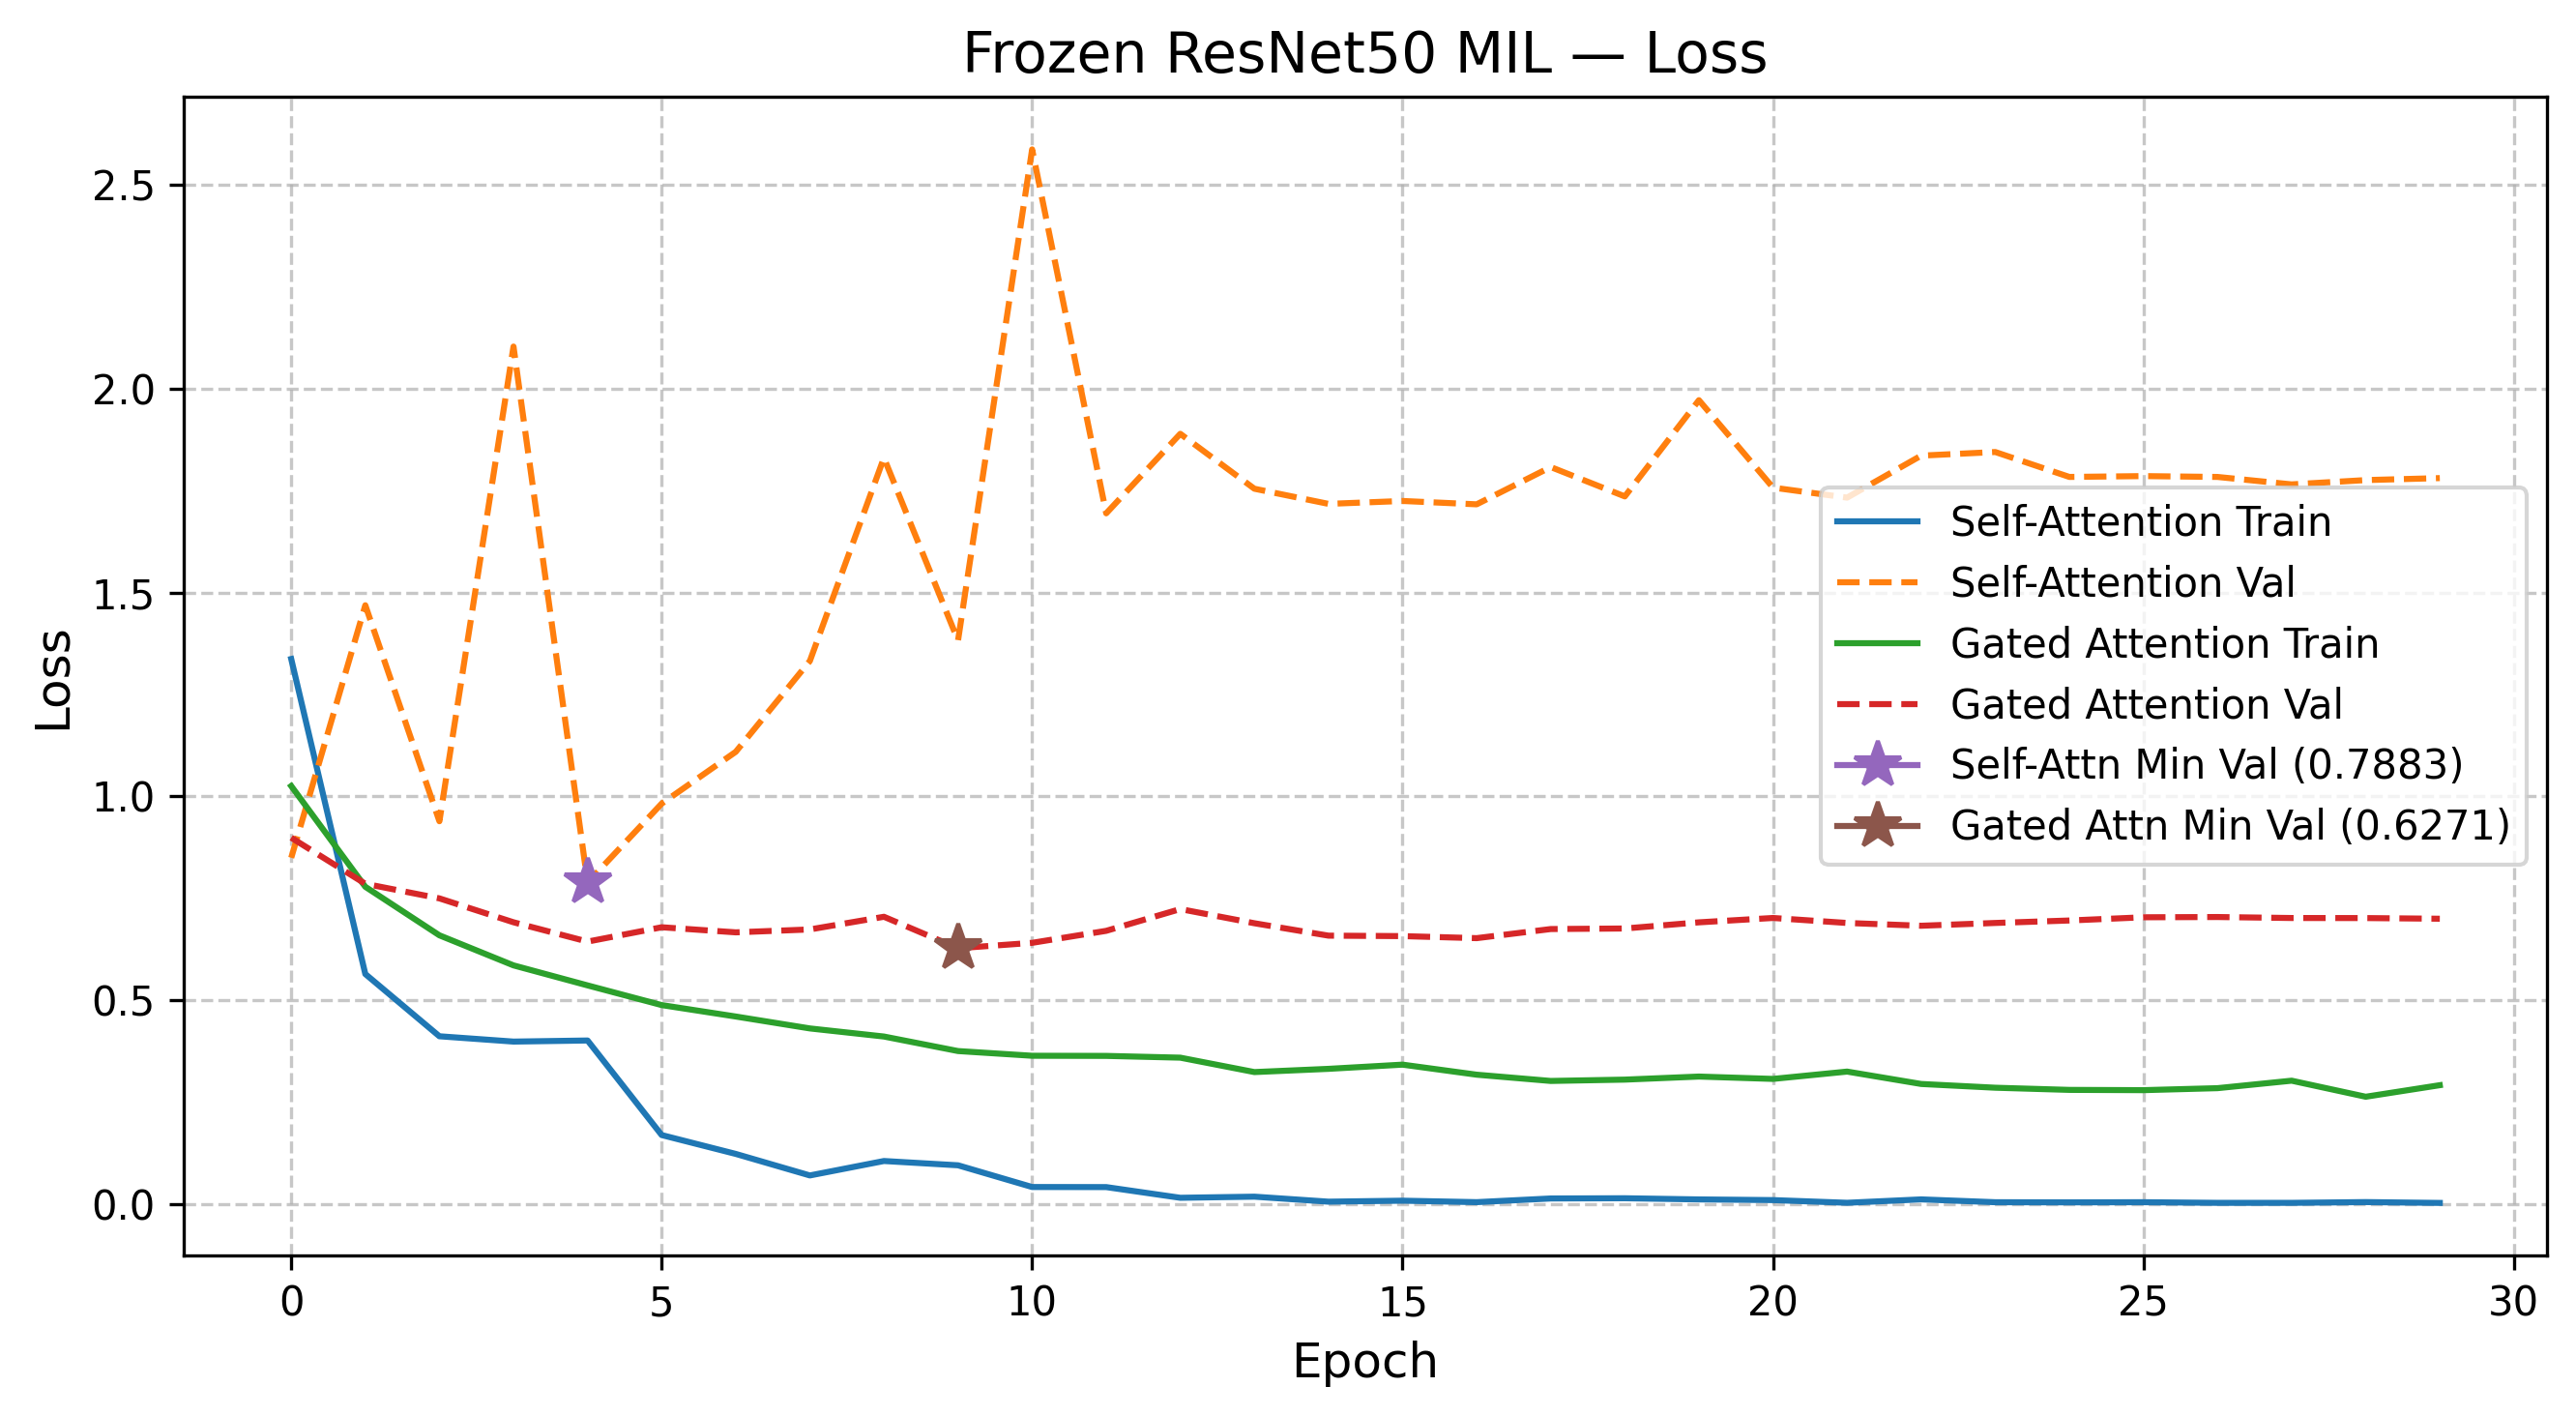
\includegraphics[width=0.31\textwidth]{mil_frozen_loss.png} &
  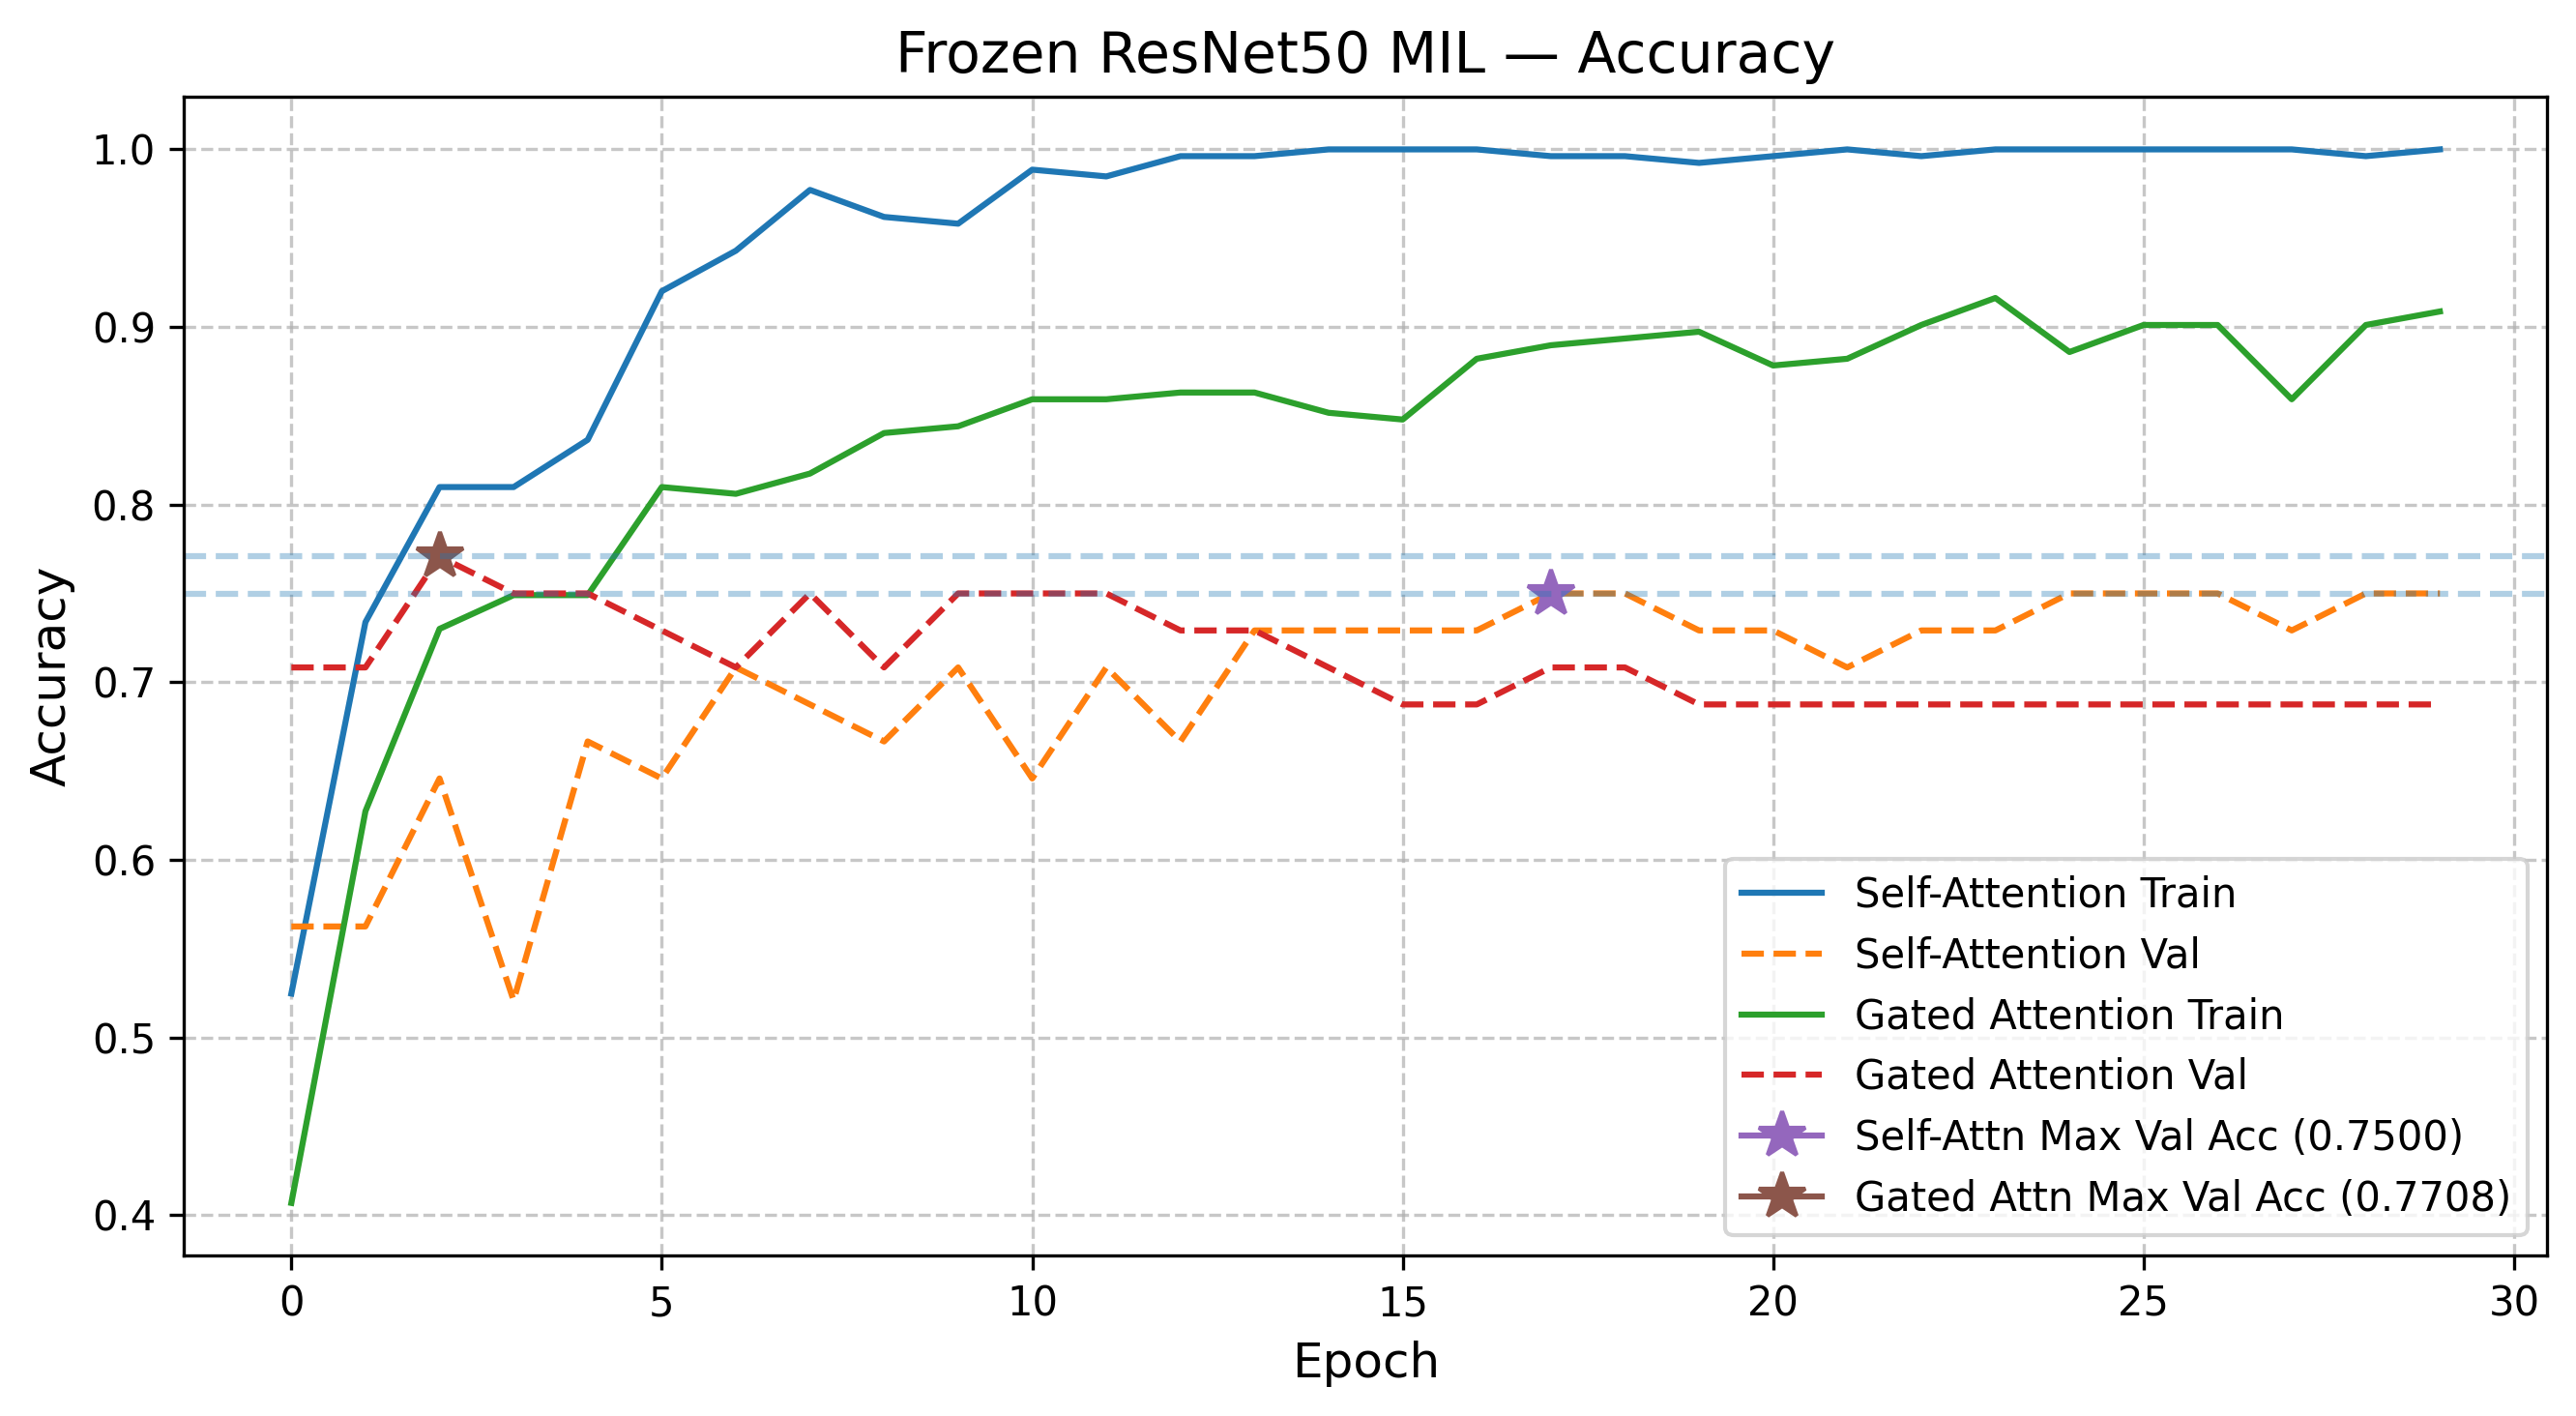
\includegraphics[width=0.31\textwidth]{mil_frozen_accuracy.png} &
  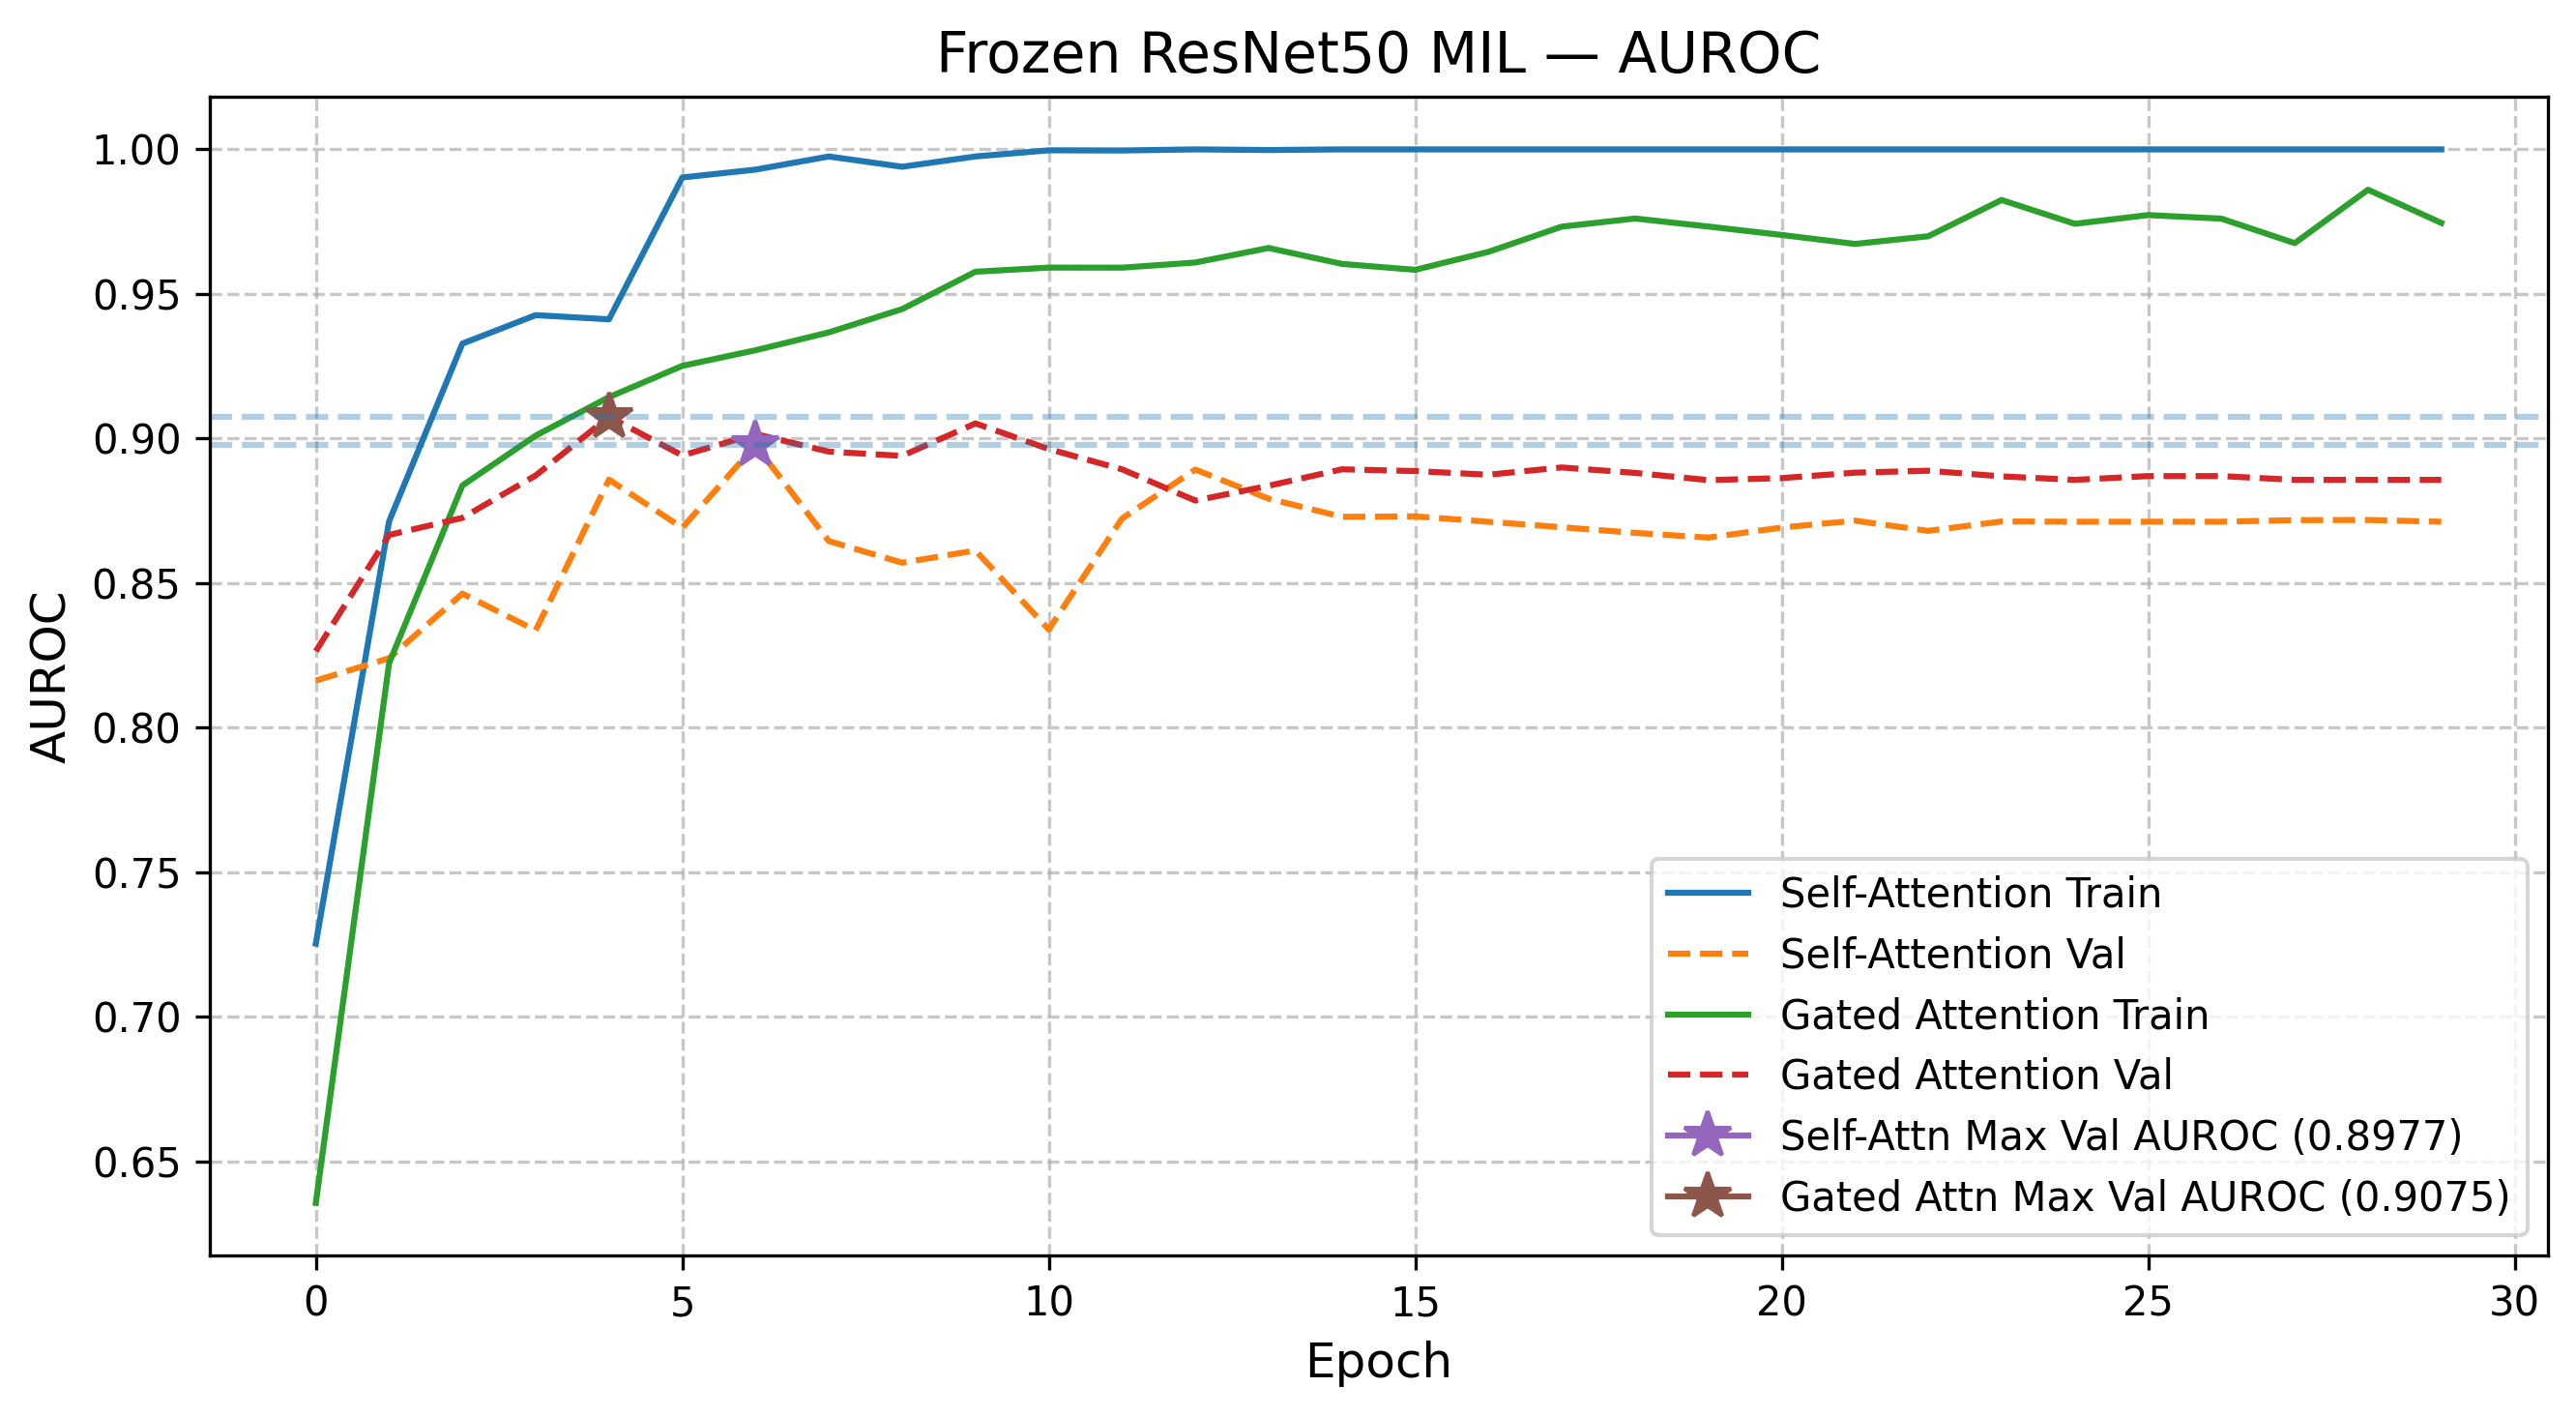
\includegraphics[width=0.31\textwidth]{mil_frozen_auc.png}
\end{tabular}
\caption{\textbf{Frozen MIL training curves} for both self-attention and gated attention aggregators. Loss (left), Accuracy (centre), and AUROC (right). Gated attention converges more stably and achieves consistently higher validation accuracy. Stars mark the best validation epoch per model.}
\label{fig:frozen_curves}
\end{figure}

\begin{figure}[h]
\centering
\begin{tabular}{cc}
  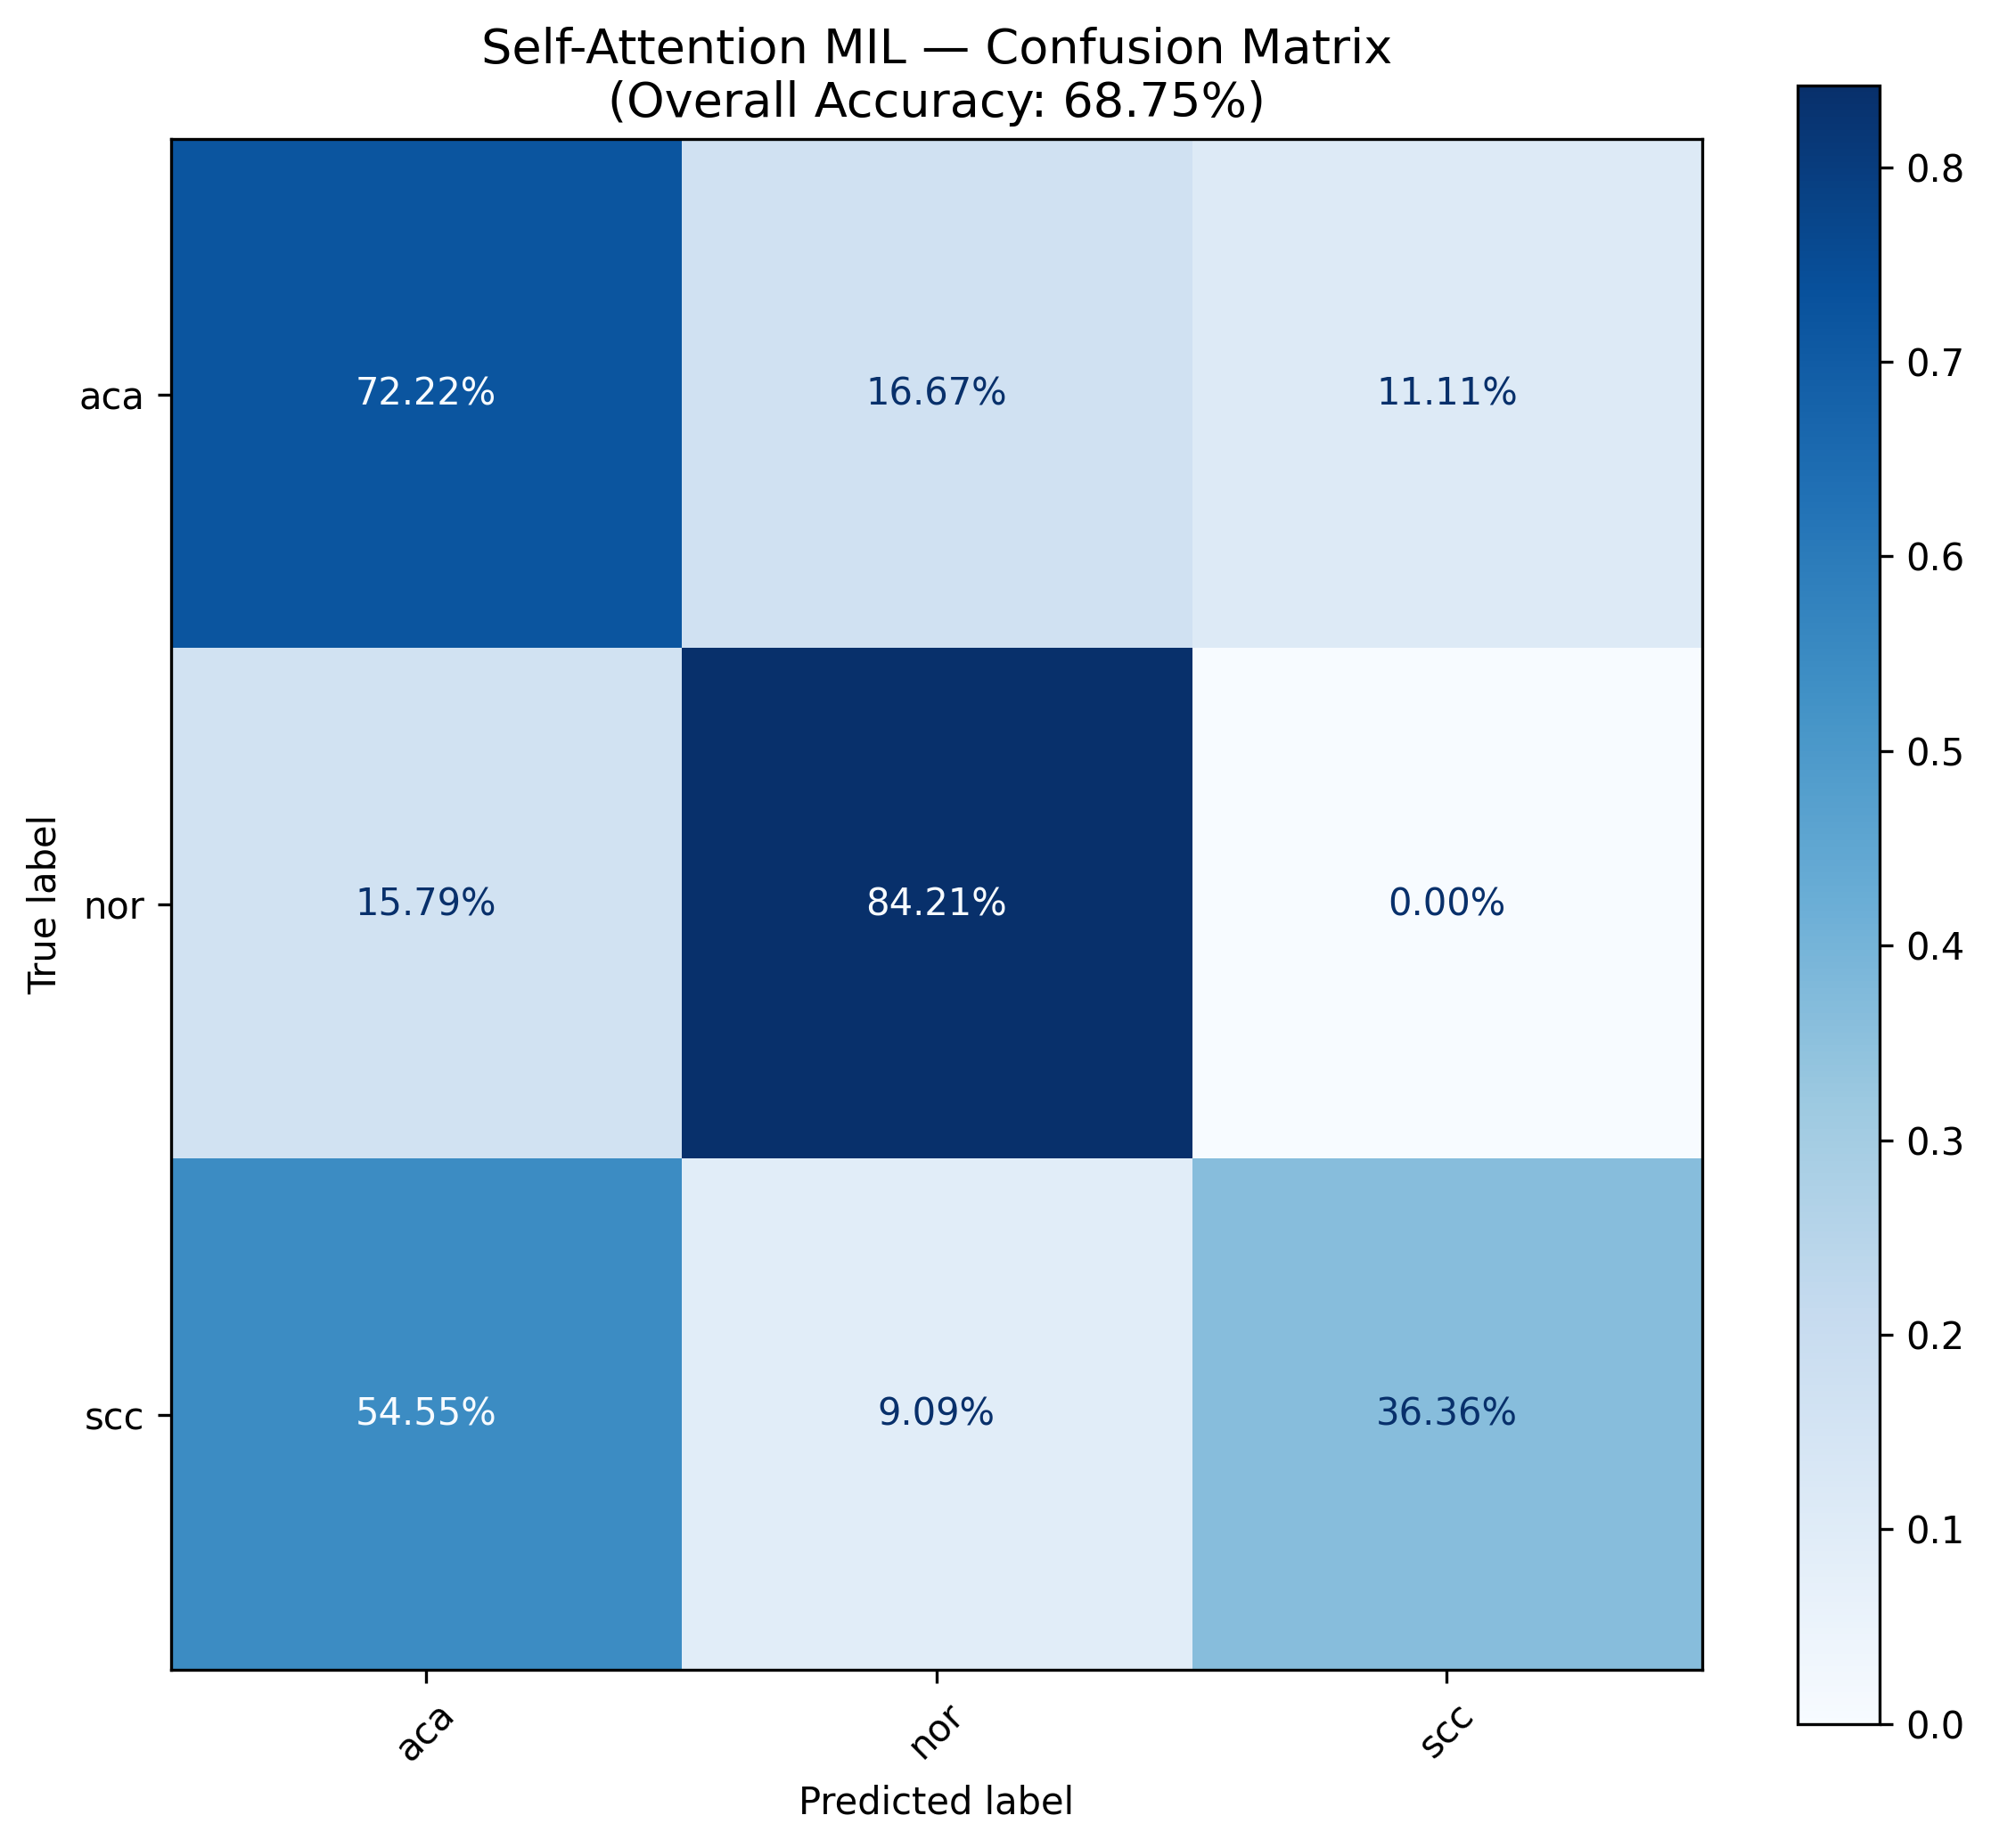
\includegraphics[width=0.42\textwidth]{self_attention_mil_confusion_matrix.png} &
  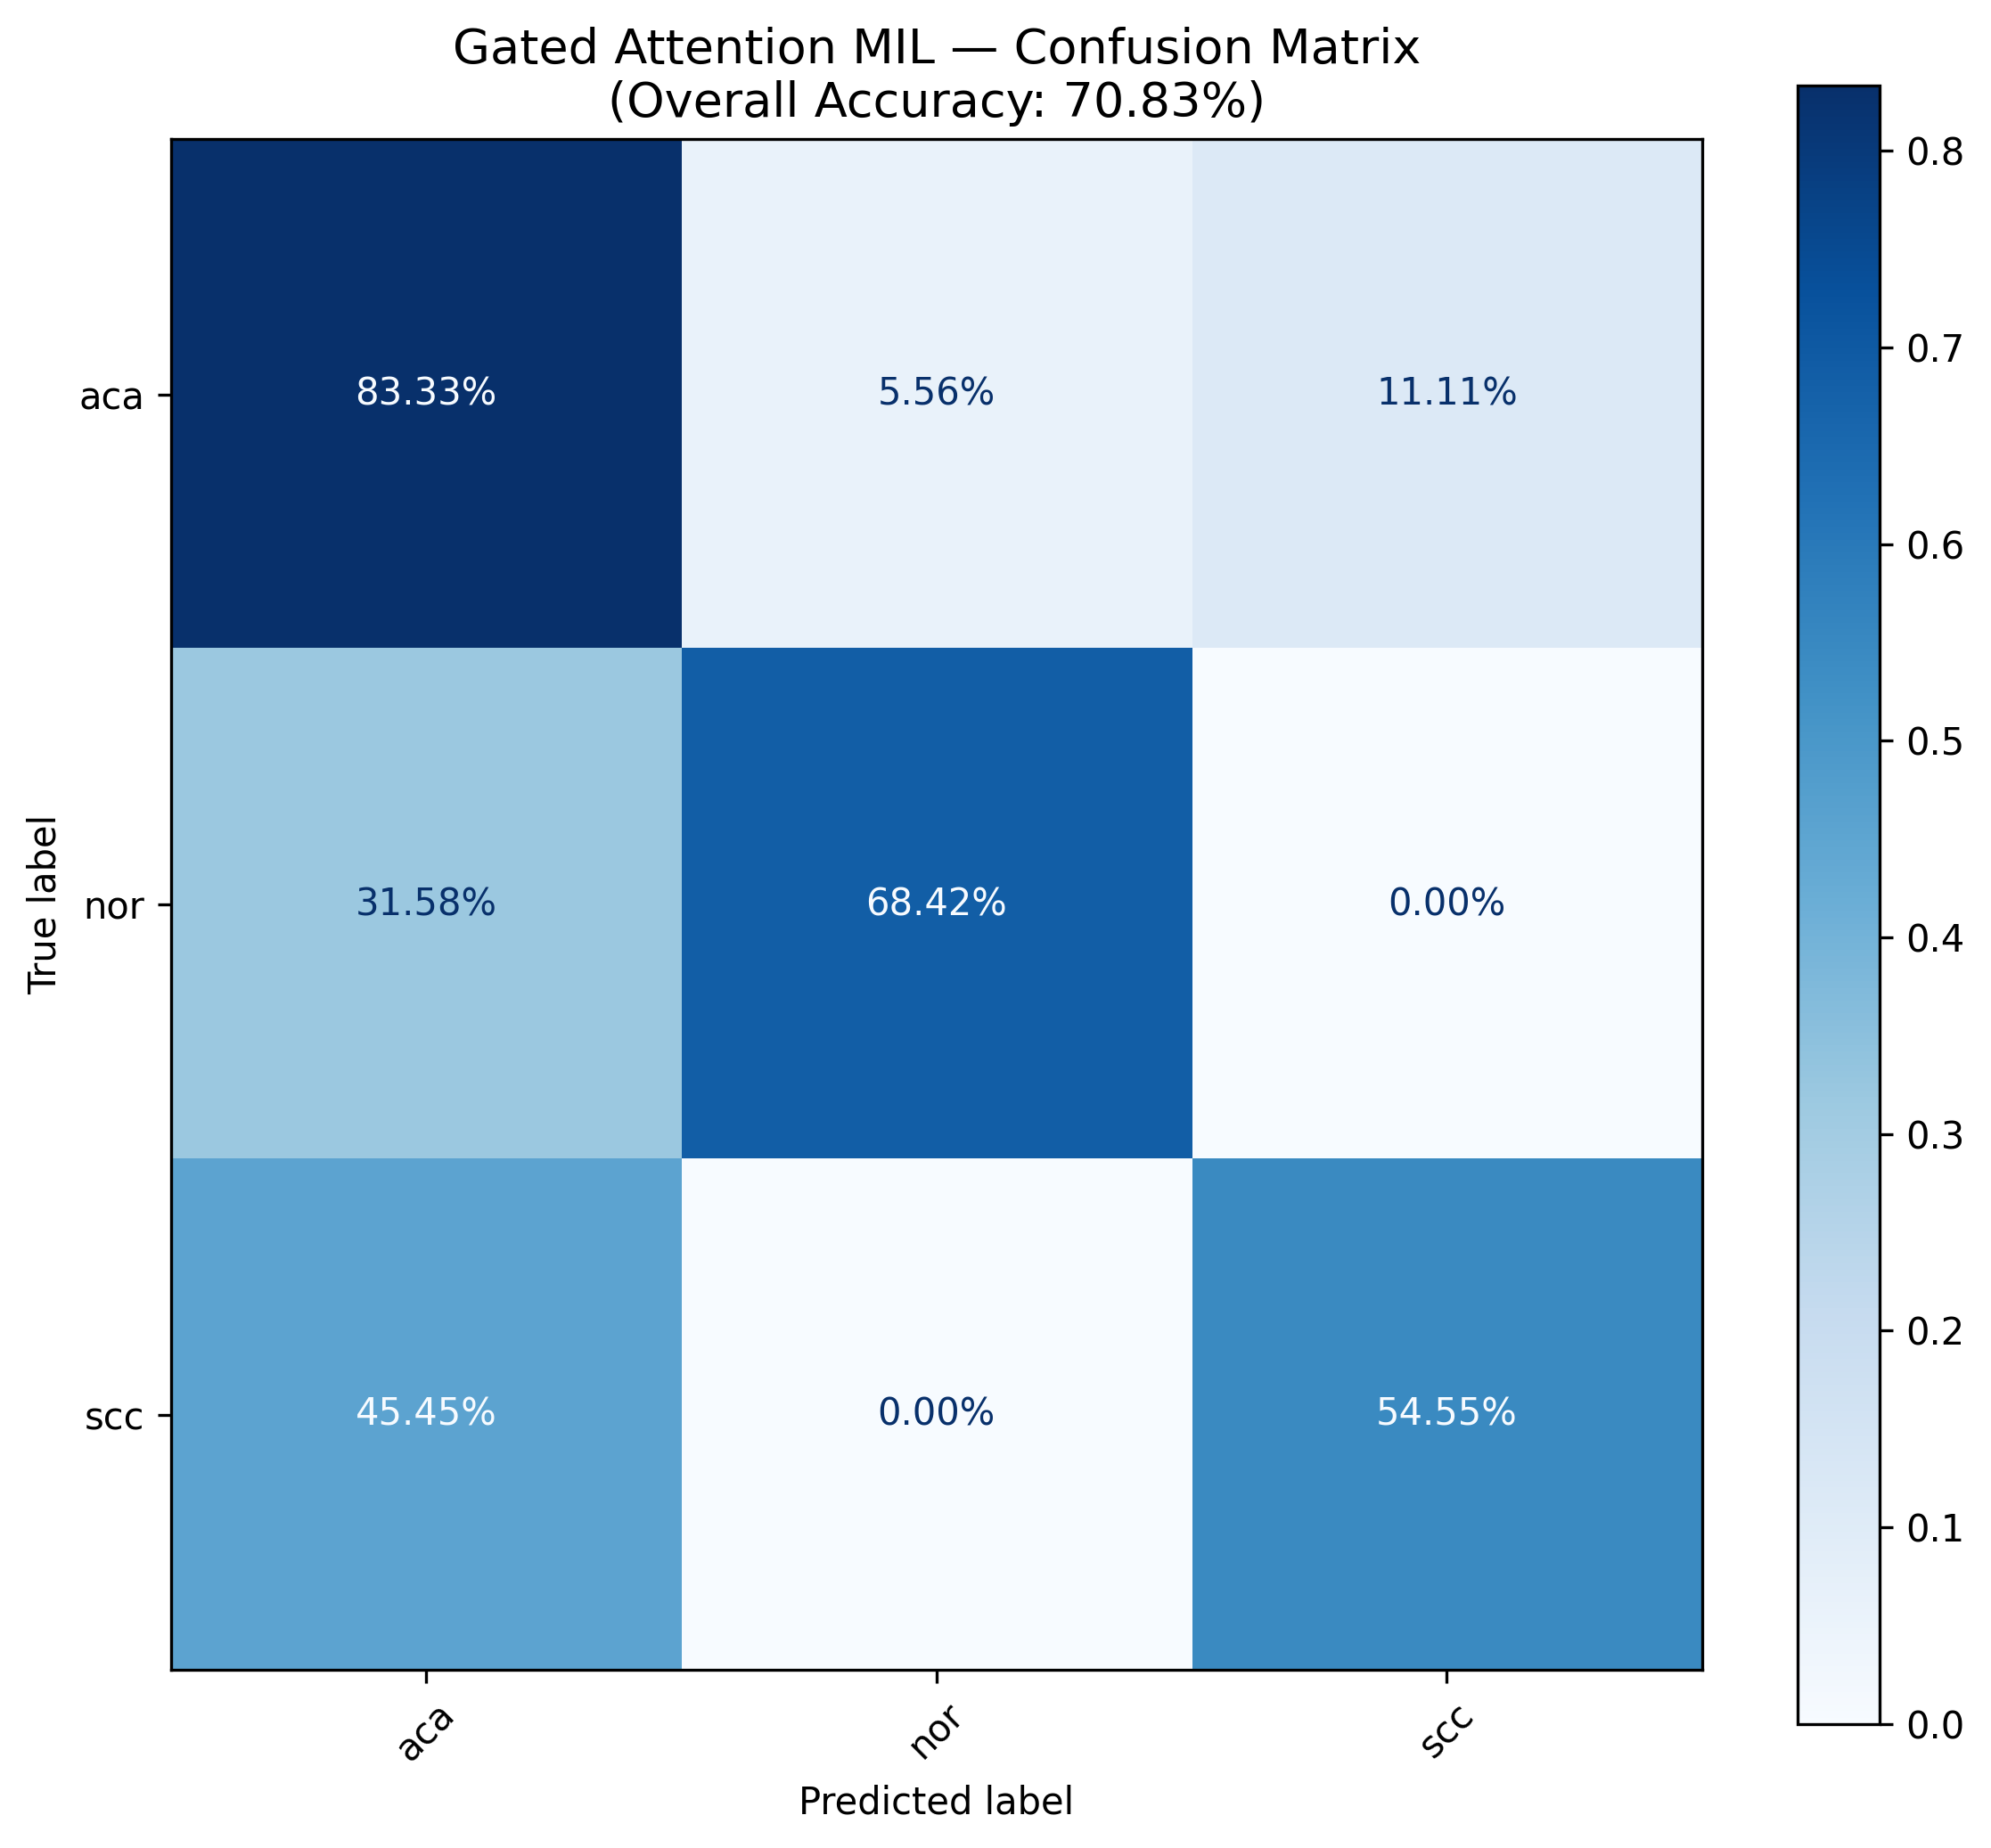
\includegraphics[width=0.42\textwidth]{gated_attention_mil_confusion_matrix.png}
\end{tabular}
\caption{\textbf{Frozen MIL normalized confusion matrices (per-class recall).} Self-Attention (left): SCC recall collapses to 36\%, indicating overfitting or insufficient feature discriminability for squamous morphology. Gated Attention (right): SCC recall improves to 55\%, NOR precision reaches 93\%; gating's sparse per-patch suppression is better suited to this small dataset.}
\label{fig:frozen_cm}
\end{figure}

% -----------------------------------------------------------------------
\subsection*{C\quad End-to-End MIL — Training Curves and Attention Visualization}
% -----------------------------------------------------------------------

\begin{figure}[h]
\centering
\begin{tabular}{ccc}
  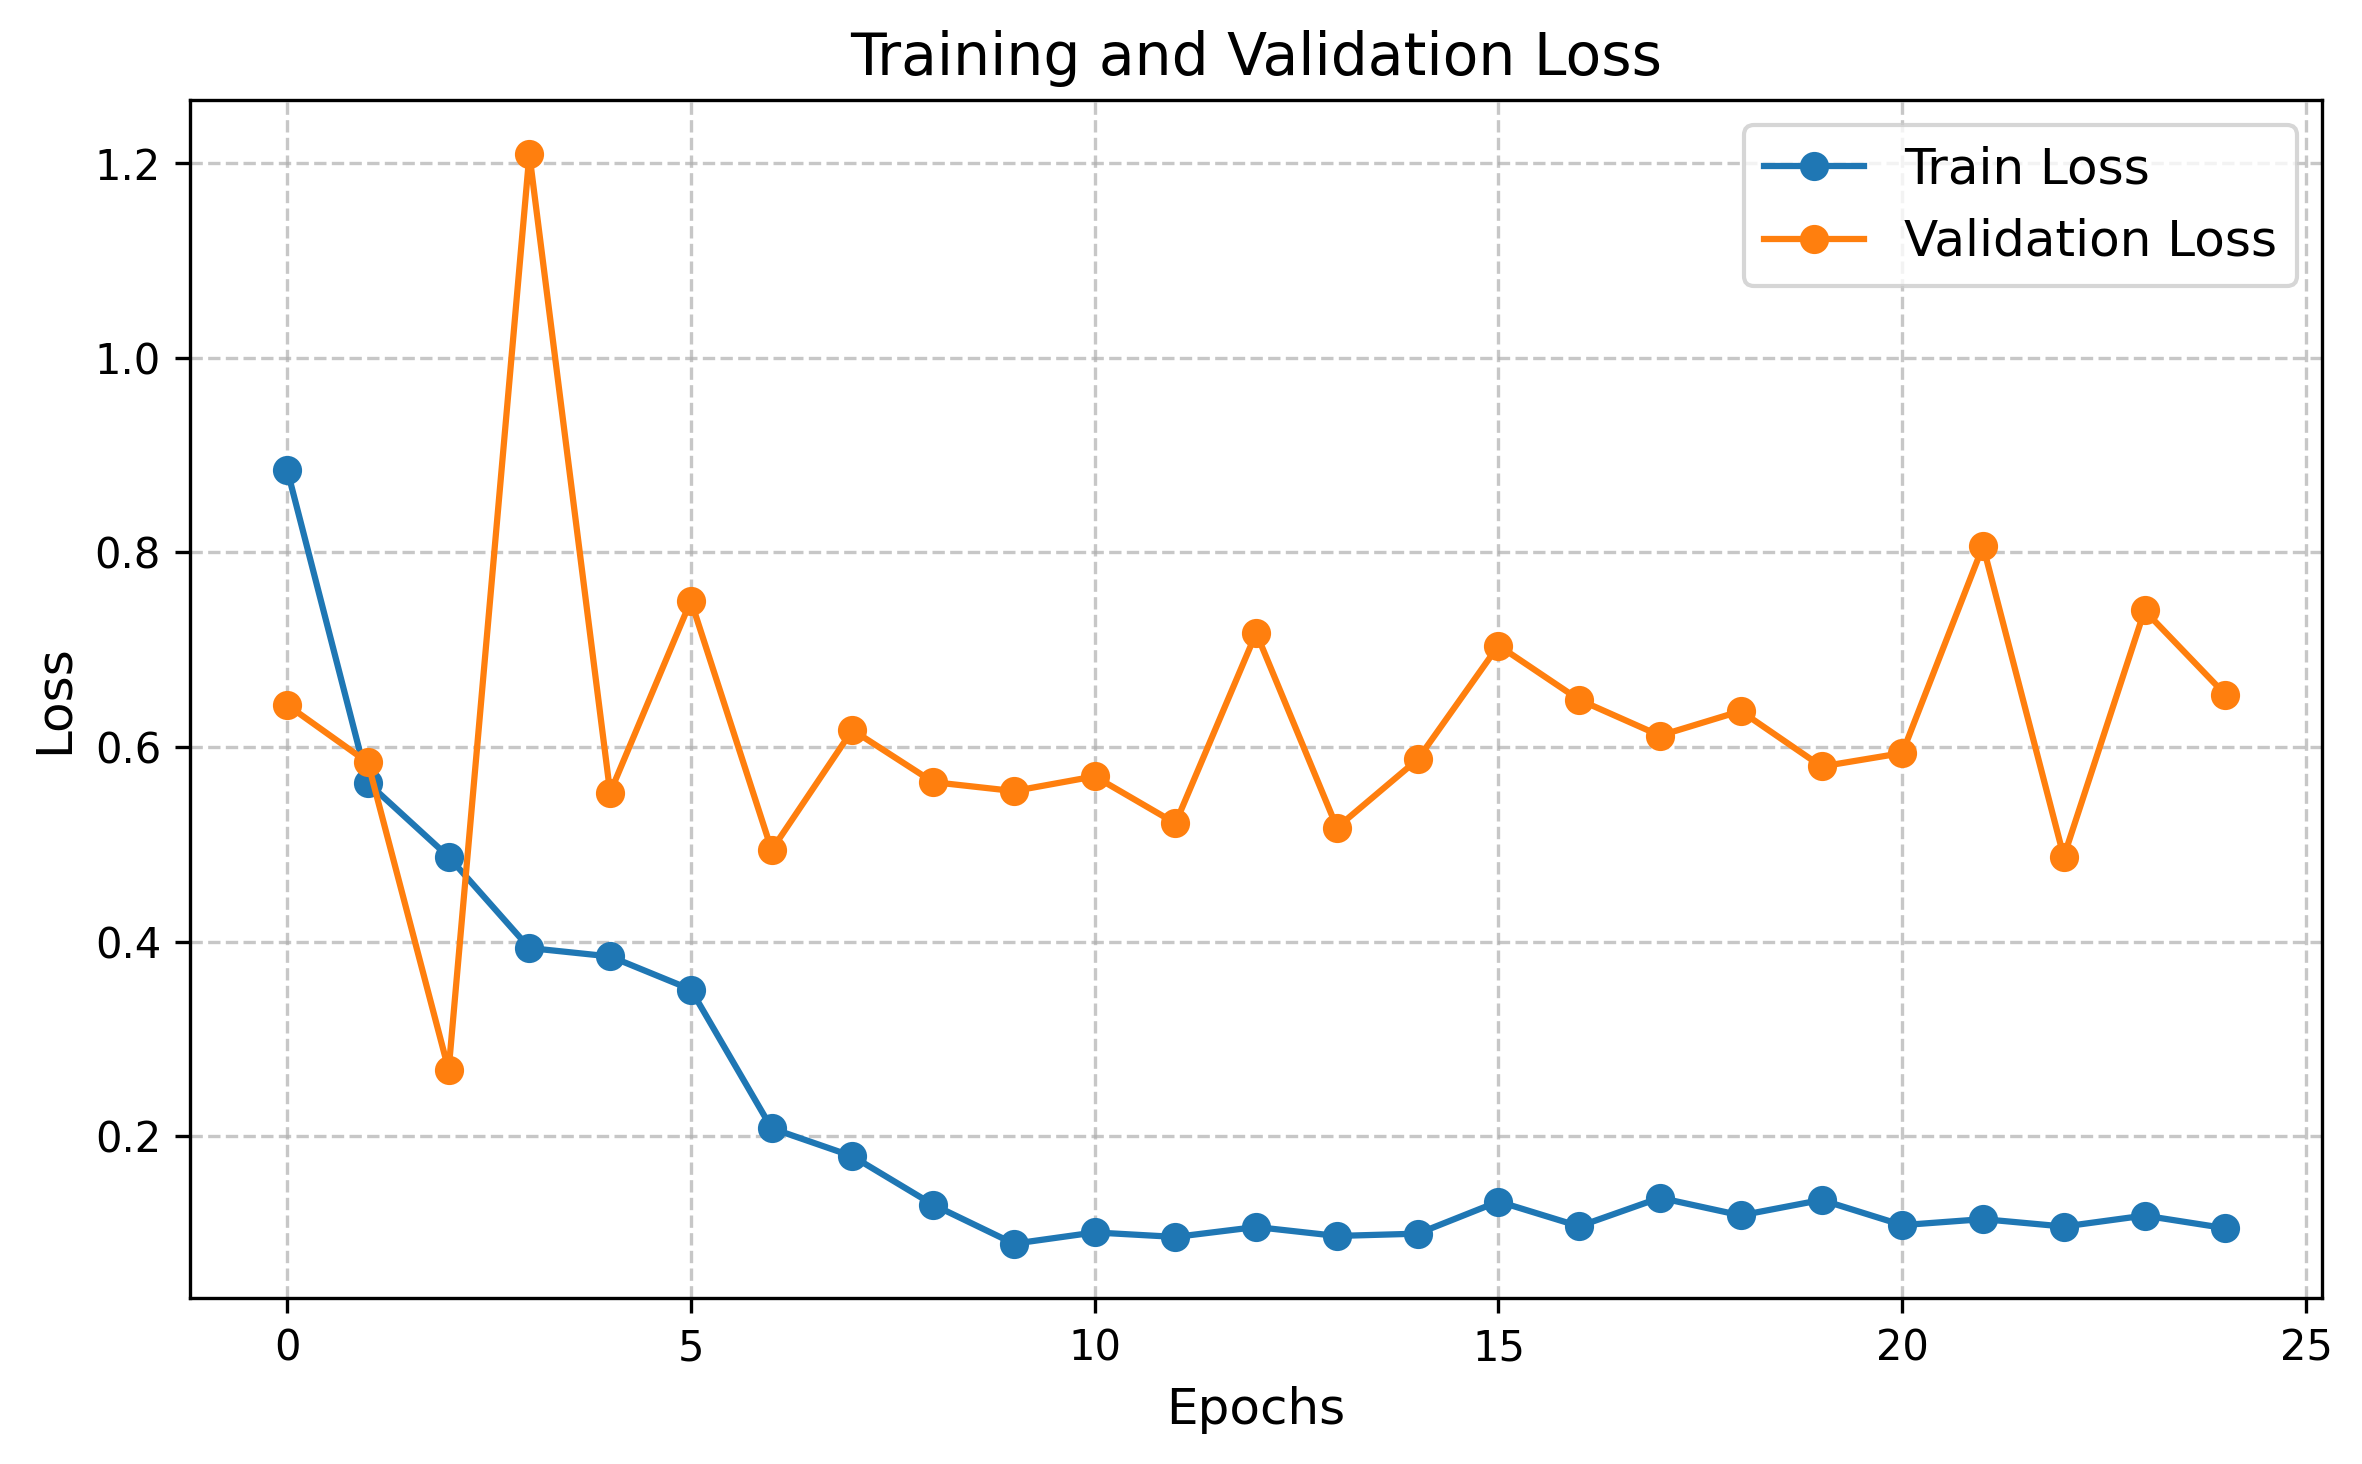
\includegraphics[width=0.31\textwidth]{mil_baseline_loss.png} &
  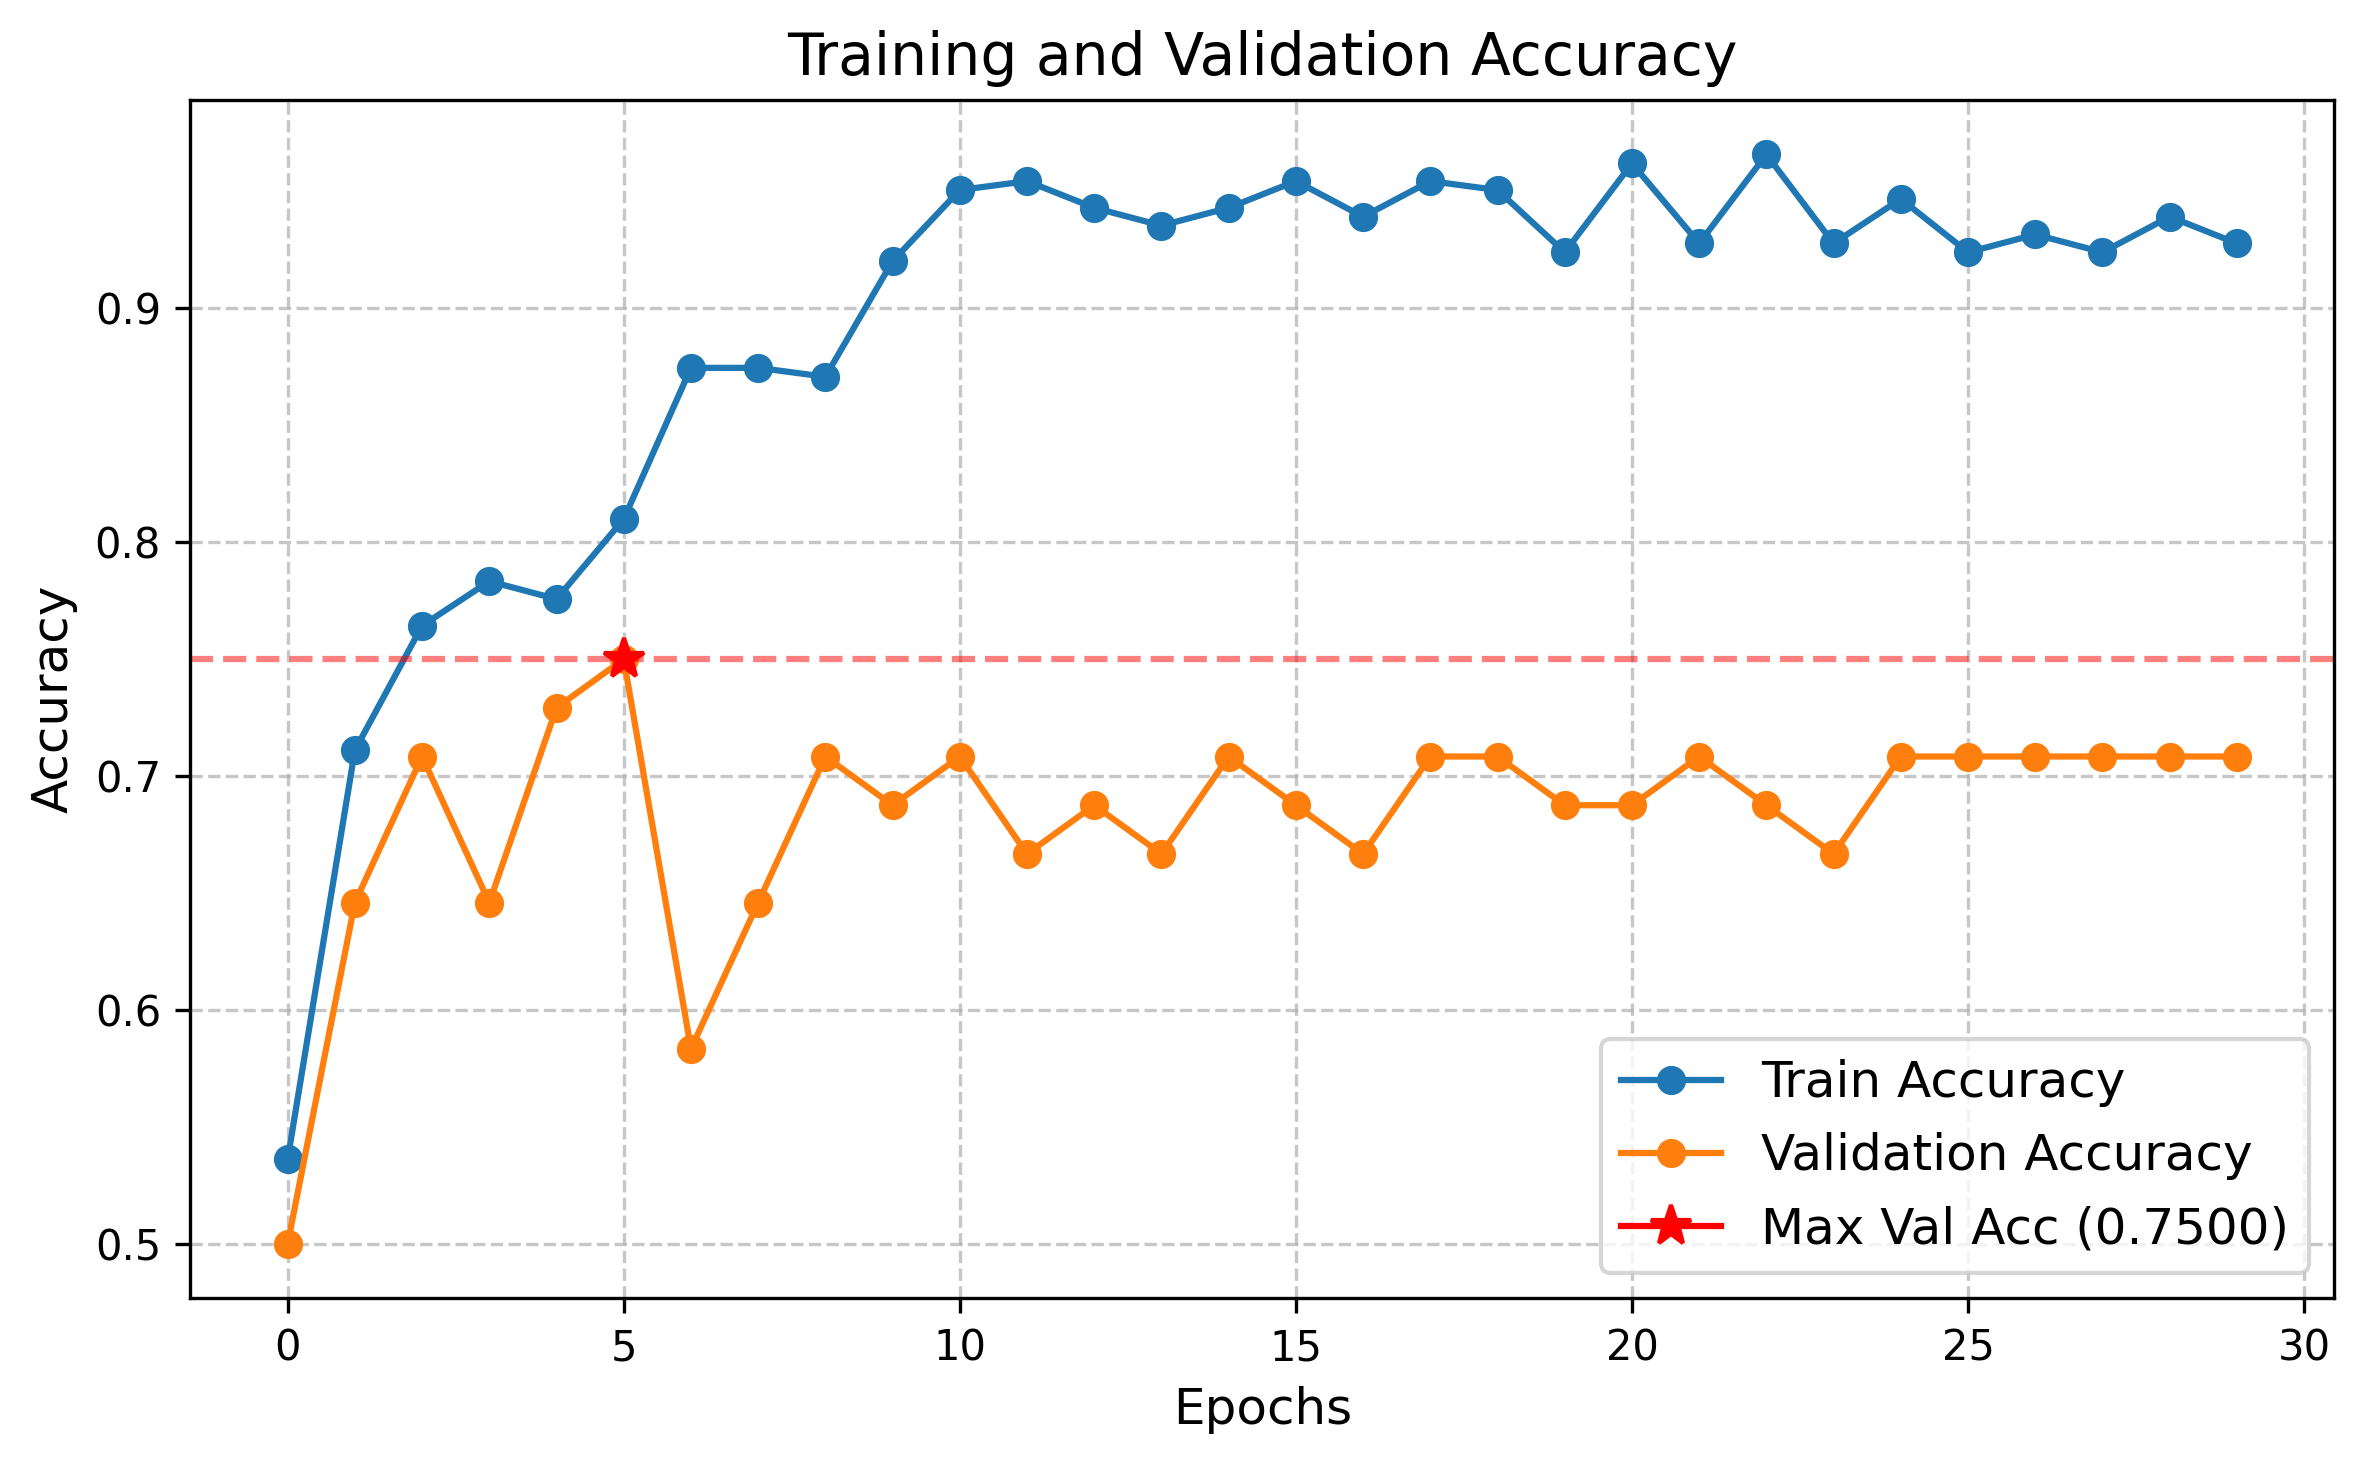
\includegraphics[width=0.31\textwidth]{mil_baseline_accuracy.png} &
  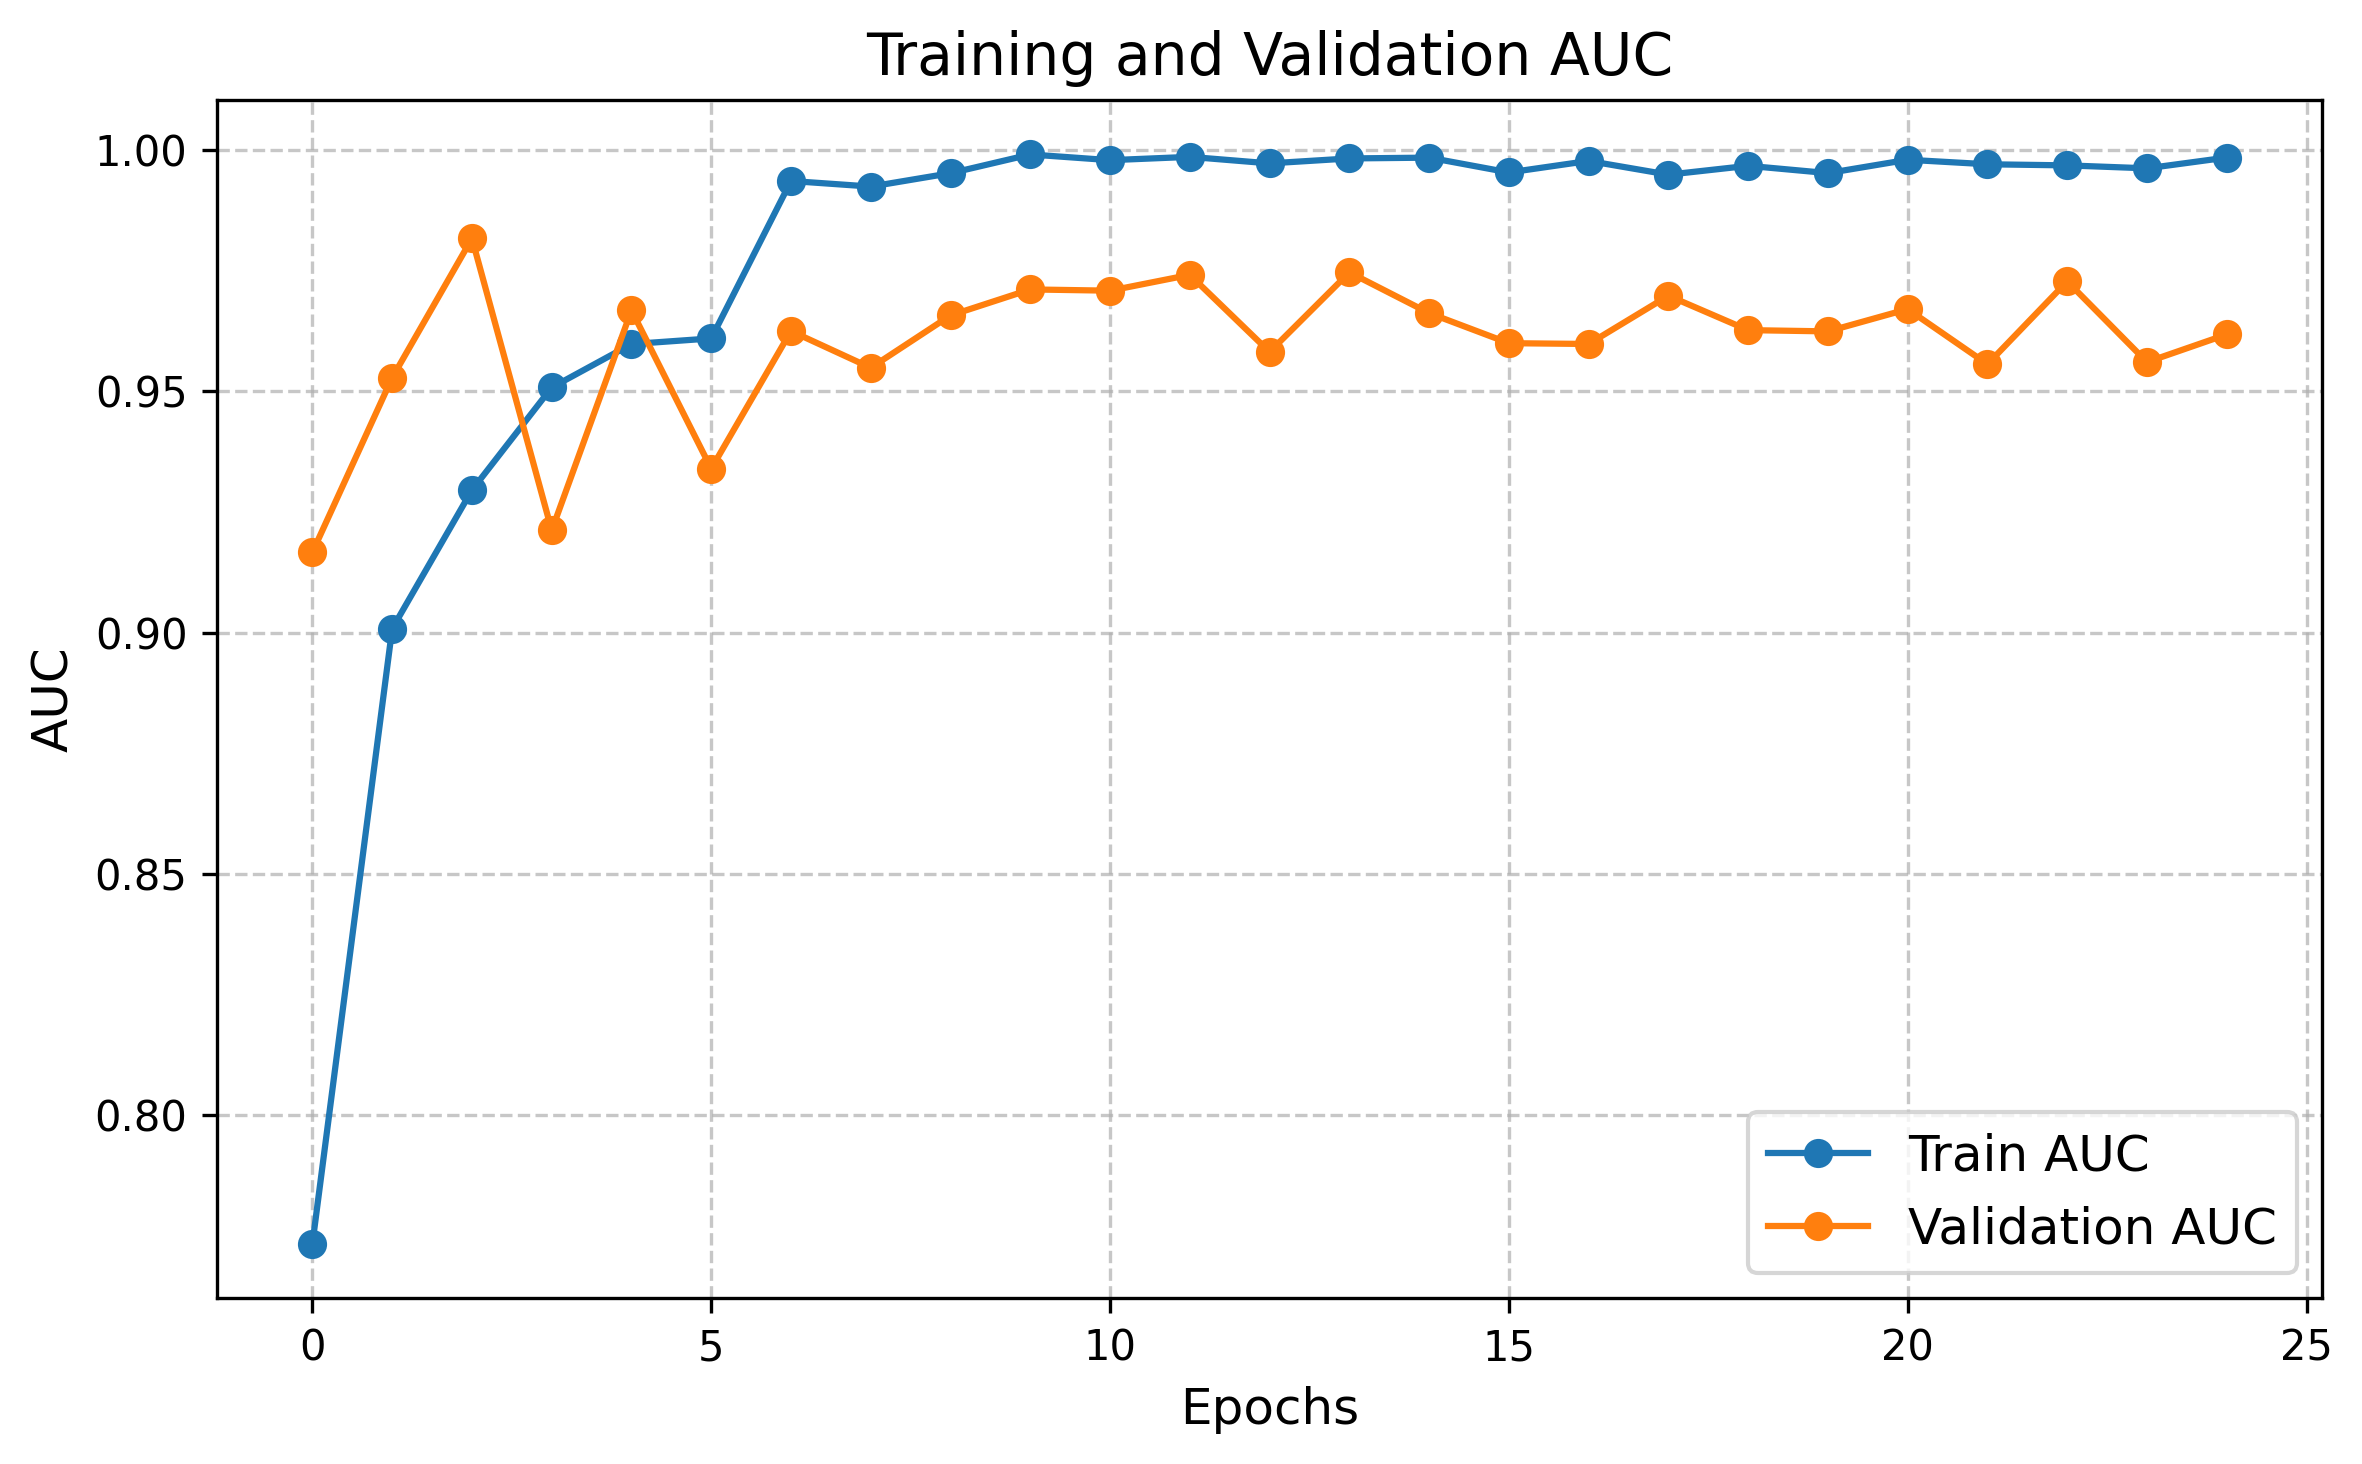
\includegraphics[width=0.31\textwidth]{mil_baseline_auc.png}
\end{tabular}
\caption{\textbf{End-to-end MIL training curves.} Training is noisier than the CNN baseline due to the weak bag-level supervision signal and joint backbone optimization. AUROC stabilizes at a higher level than accuracy, consistent with well-calibrated probability outputs. Stars mark the best validation epoch.}
\label{fig:e2e_mil_curves}
\end{figure}

\begin{figure}[h]
\centering
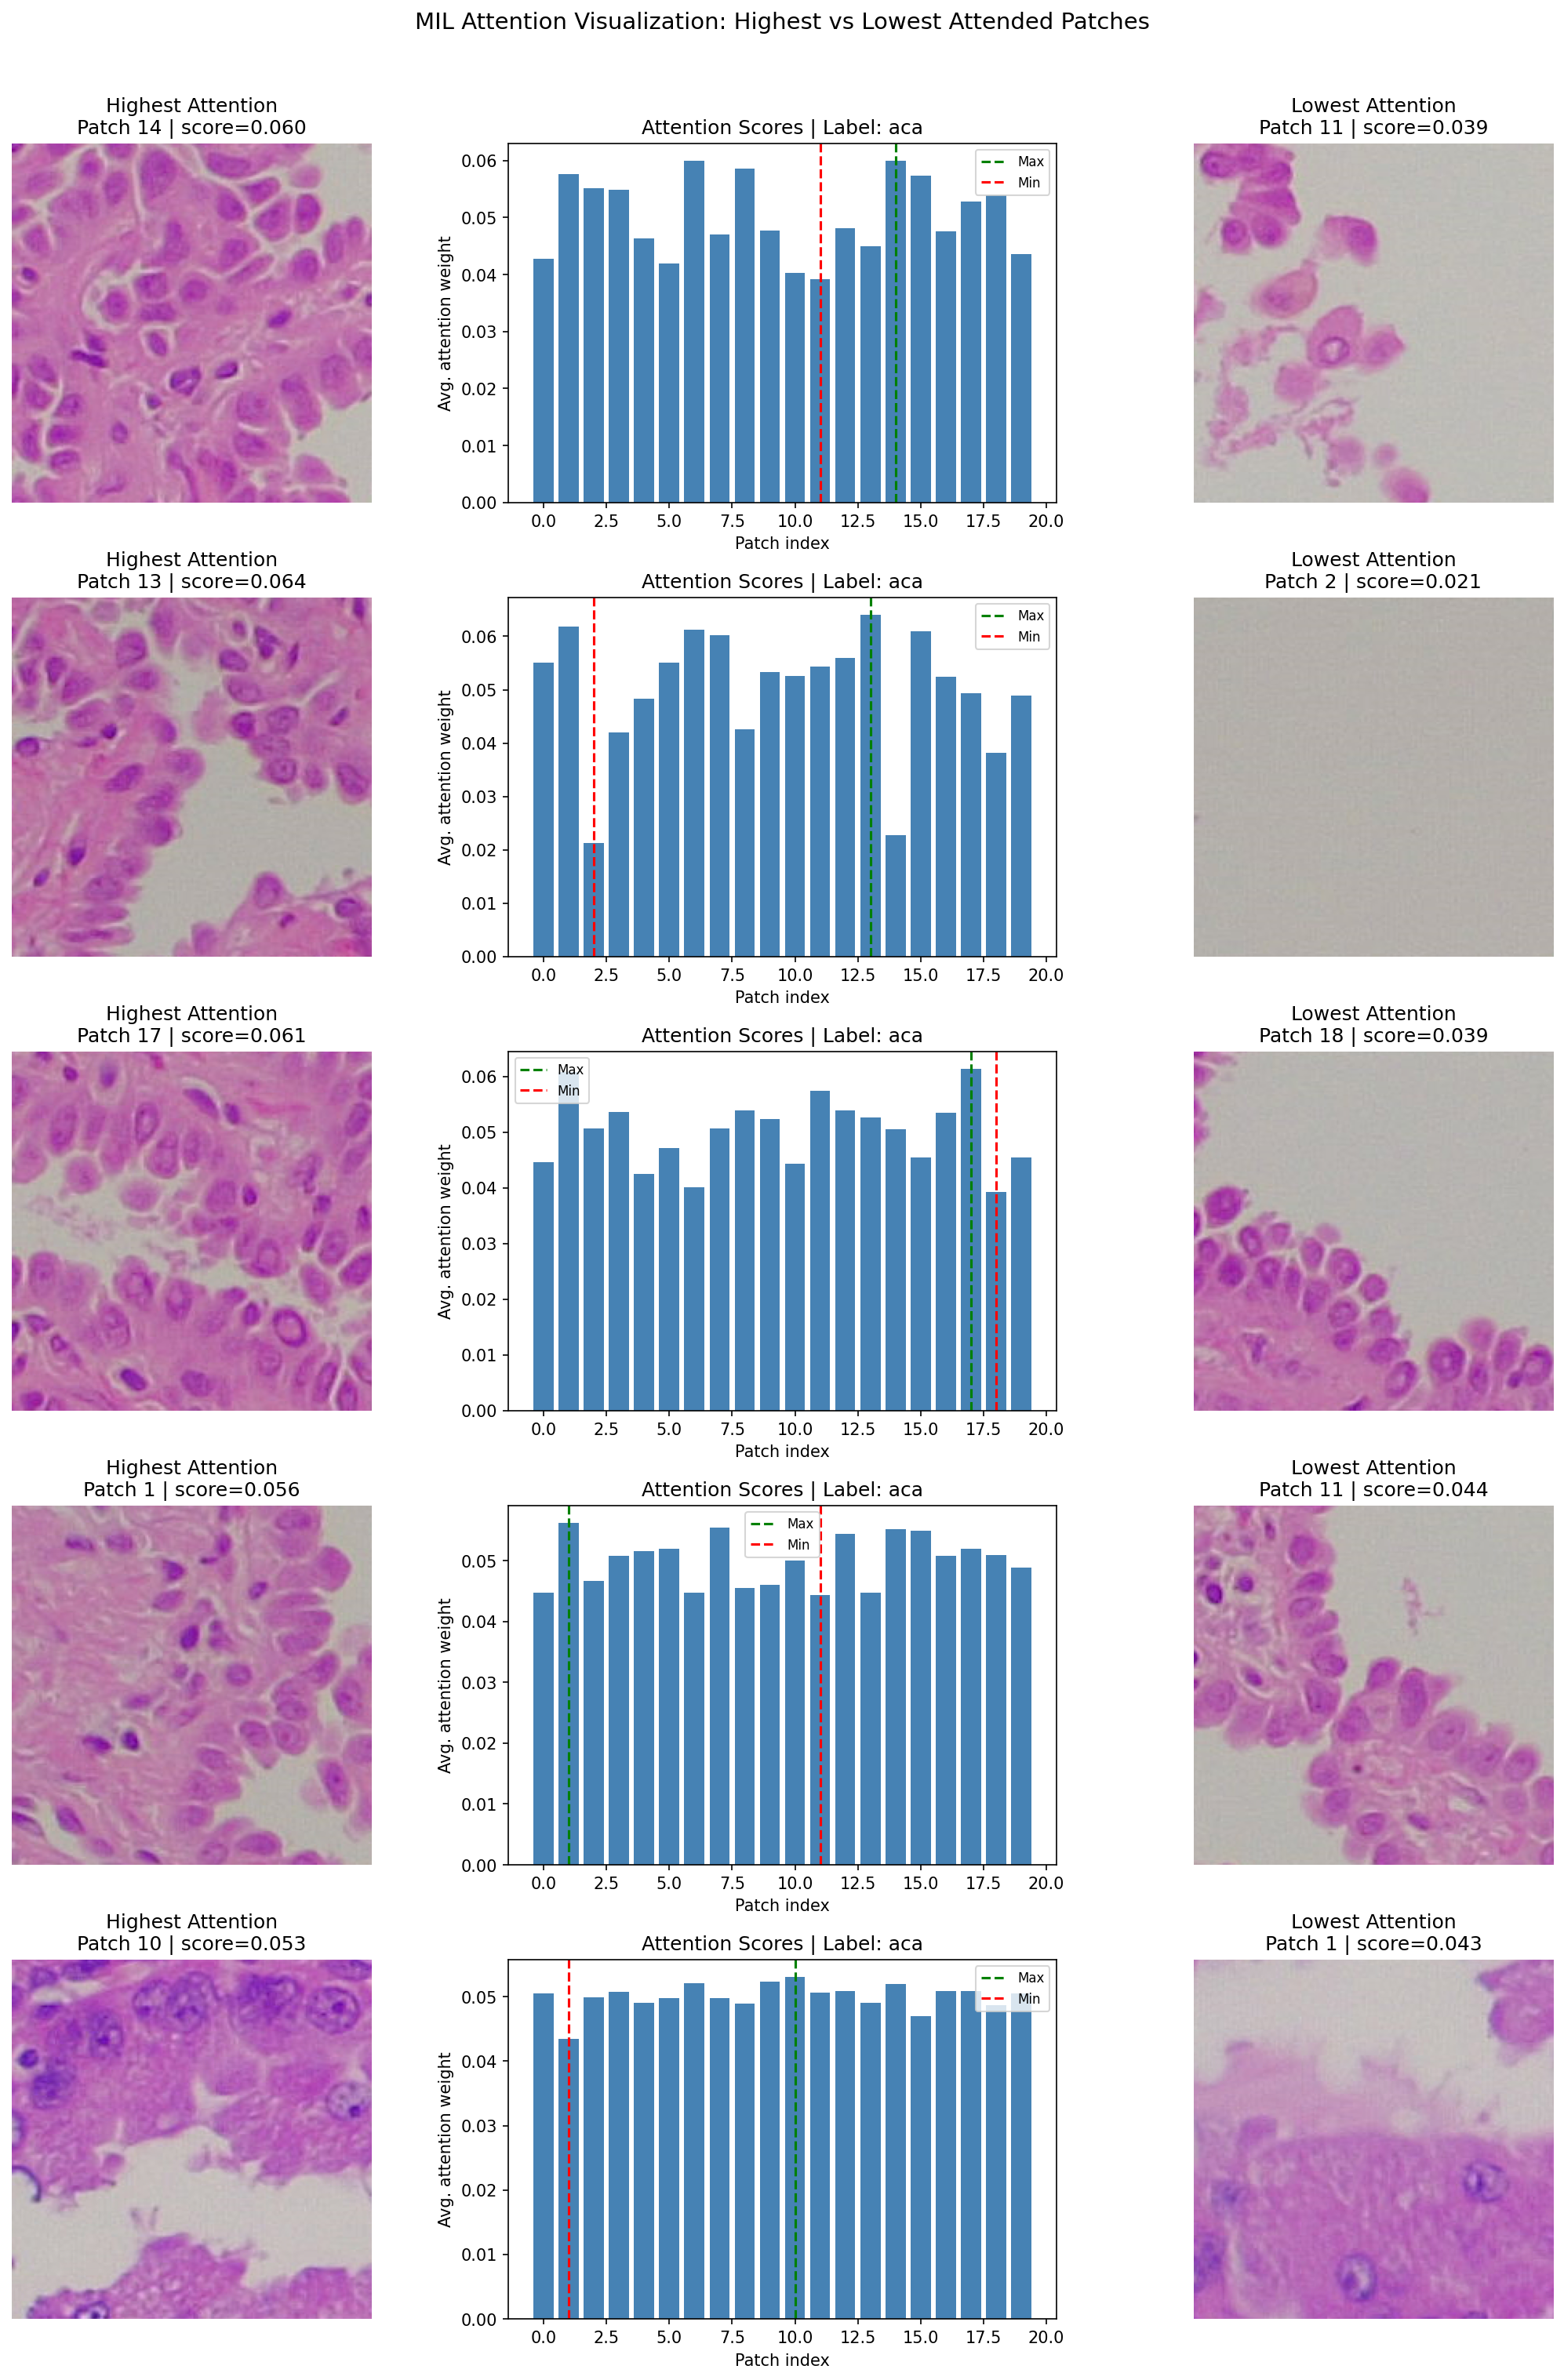
\includegraphics[width=0.92\textwidth]{mil_attention_viz.png}
\caption{\textbf{End-to-end MIL attention visualization.} For each validation bag: the highest-attention patch (left column), the per-patch attention score distribution (centre), and the lowest-attention patch (right column). The model consistently assigns high attention to patches containing dense nuclei and glandular structures, and low attention to predominantly stromal or background regions — confirming clinically meaningful patch selection.}
\label{fig:attn_viz}
\end{figure}

\begin{figure}[h]
\centering
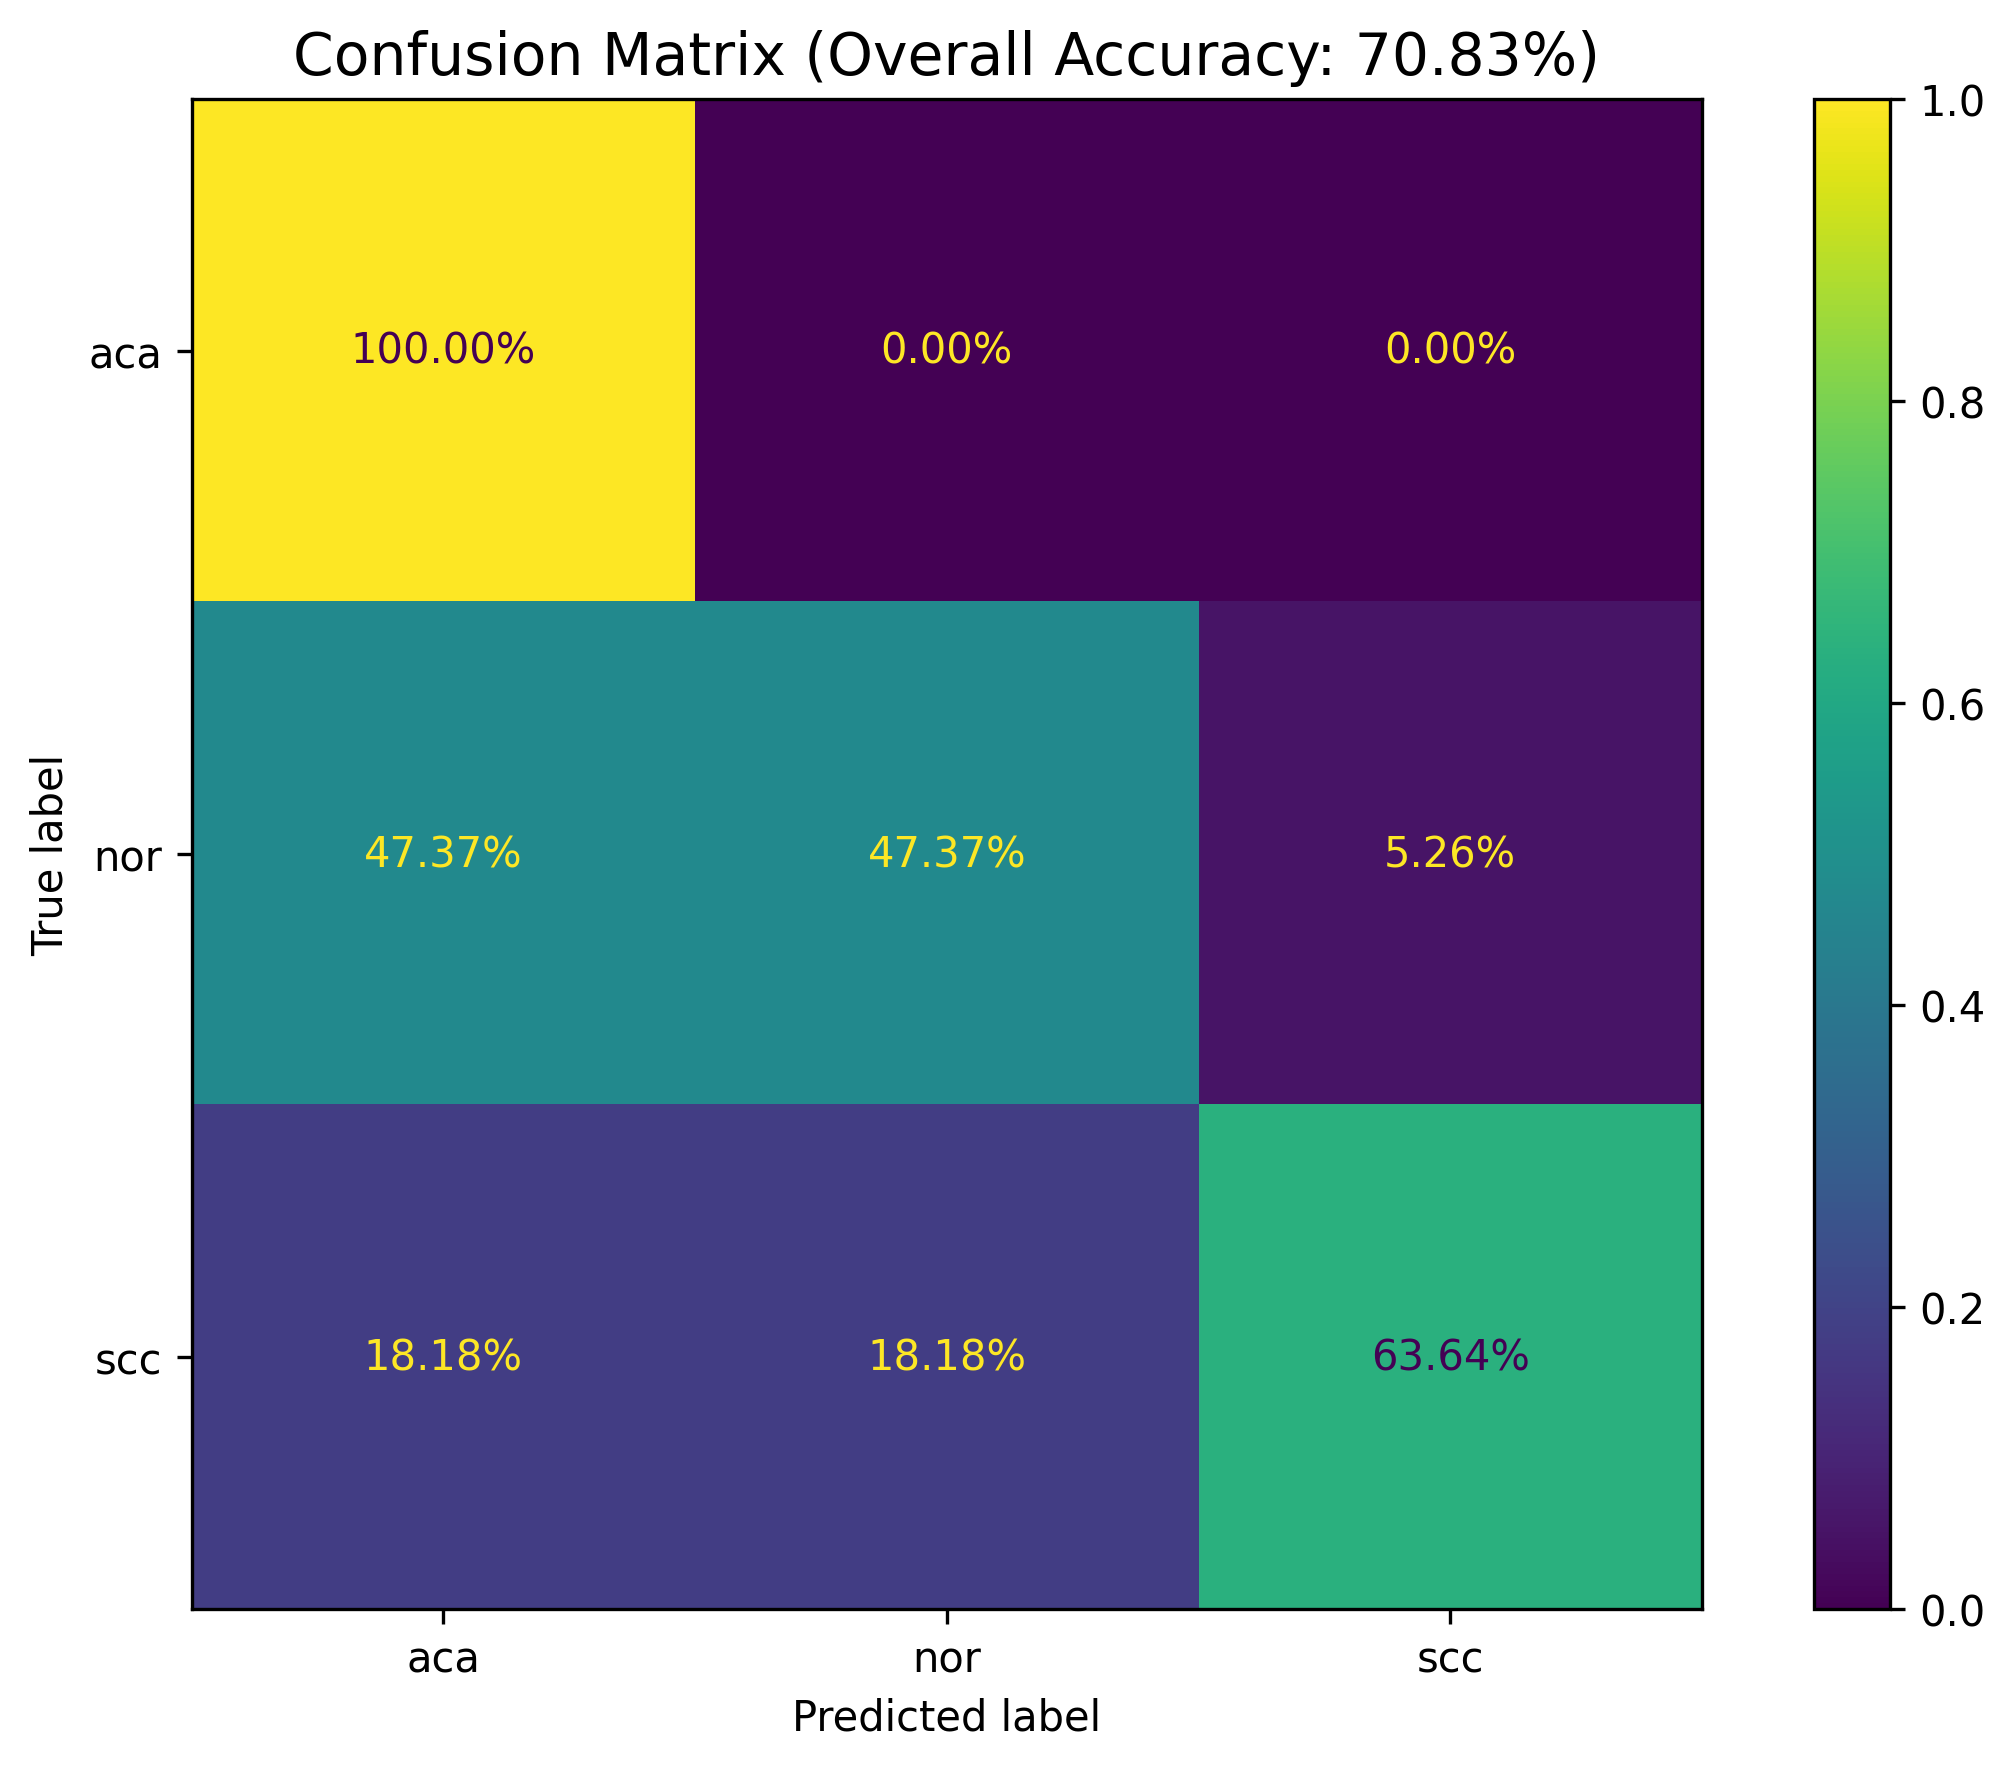
\includegraphics[width=0.5\textwidth]{mil_baseline_confusion_matrix.png}
\caption{\textbf{End-to-end MIL — normalized confusion matrix.} Overall accuracy 70.8\%. ACA and NOR are reasonably well separated; SCC is the most confused class (frequently predicted as ACA), consistent with morphological overlap at 20$\times$ and the absence of patch-level supervision.}
\label{fig:e2e_mil_cm}
\end{figure}

% -----------------------------------------------------------------------
\subsection*{D\quad Bag Construction Comparison}
% -----------------------------------------------------------------------

\begin{table}[h]
\centering
\caption{Bag construction comparison: paper vs.\@ our implementations.}
\setlength{\tabcolsep}{6pt}
\begin{tabular}{lccc}
\toprule
Property & Paper MIL & Our End-to-End MIL & Our Frozen MIL \\
\midrule
Patch size       & 224$\times$224   & 224$\times$224   & 224$\times$224 \\
Patches per bag  & 20               & 20               & 35 (5$\times$7 grid) \\
Selection method & Random crop      & Random crop      & Deterministic grid \\
Source image     & Full-res (1200$\times$1600)  & Full-res (1200$\times$1600) & Full-res (1200$\times$1600) \\
Stochastic bag?  & Yes (per epoch)  & Yes (per epoch)  & No (cached offline) \\
\bottomrule
\end{tabular}
\label{tab:bag_construction}
\end{table}

\noindent The frozen MIL uses a larger, deterministic bag (35 patches from a 5$\times$7 grid) to enable offline embedding extraction. This guarantees exhaustive spatial coverage and perfectly reproducible evaluation, at the cost of including more uninformative patches (stroma, background) — which the gated attention head learns to suppress.

% -----------------------------------------------------------------------
\subsection*{E\quad Environment and Reproducibility Details}
% -----------------------------------------------------------------------

\begin{table}[h]
\centering
\caption{Training environment.}
\setlength{\tabcolsep}{8pt}
\begin{tabular}{ll}
\toprule
Component & Details \\
\midrule
OS                  & WSL2 (Fedora) \\
Python              & 3.13 \\
Framework           & PyTorch 2.x (primary), TensorFlow 2.x (TF baseline) \\
GPU                 & NVIDIA GPU (detected via \texttt{torch.cuda.is\_available()}) \\
CUDA                & 12.x \\
Key packages        & torchvision, torchmetrics, scikit-learn, albumentations \\
Optimizer           & Adam, lr\,=\,1e-4 (CNN), lr\,=\,1e-3 (MIL heads) \\
LR schedule         & ReduceLROnPlateau (patience 2--3, factor 0.1--0.5) \\
Early stopping      & Best val loss checkpoint saved \\
Augmentations       & Random crop, H-flip, V-flip, grid distortion, & \\
                    & $\gamma$, brightness/contrast, HSV jitter \\
\bottomrule
\end{tabular}
\label{tab:env}
\end{table}

\noindent\textbf{Resolved issues during experimentation:}
\begin{itemize}
\item CUDA/cuDNN library path resolution under WSL for TensorFlow GPU detection.
\item TensorFlow–protobuf version alignment.
\item Missing default dataset path (\texttt{data/data.csv}) in baseline scripts.
\item MIL patch extraction bug: patches were incorrectly extracted from a downscaled 300$\times$400 image instead of the full 1200$\times$1600 original, discarding micro-texture detail. Fixed by removing the initial downscale step in \texttt{MIL\_LungHistDataset}.
\item \texttt{NameError} when reloading \texttt{pytorch\_mil} module before first import — resolved by ensuring import precedes \texttt{importlib.reload}.
\end{itemize}

\noindent All code, trained weights, and notebooks are publicly available at:
\url{https://github.com/skattoju/LungHist700/}

\end{document}
